\documentclass[table, 12pt]{article}
\usepackage[T1]{fontenc}
\usepackage[utf8]{inputenc}
\usepackage[english]{babel}
\usepackage{graphicx}
\usepackage{titlesec}
\usepackage{hyperref}
\usepackage[usenames,dvipsnames]{xcolor}
\usepackage{float}
\usepackage[export]{adjustbox}
\usepackage{longtable}
\usepackage{mathtools}
\usepackage[most]{tcolorbox}
\newcounter{testexample}
\usepackage{xparse}
\usepackage{subcaption}
\usepackage{amsmath}


\titleformat{\paragraph}
{\normalfont\normalsize\bfseries}{\theparagraph}{1em}{}
\titlespacing*{\paragraph}
{0pt}{3.25ex plus 1ex minus .2ex}{1.5ex plus .2ex}

\NewDocumentEnvironment{testexample}{ O{} }
{
\colorlet{colexam}{teal!60!black} % Global example color
\newtcolorbox[use counter=testexample]{testexamplebox}{%
    % Example Frame Start
    empty,% Empty previously set parameters
    title={\exampletext #1},% use \thetcbcounter to access the testexample counter text
    % Attaching a box requires an overlay
    attach boxed title to top left,
       % Ensures proper line breaking in longer titles
       minipage boxed title,
    % (boxed title style requires an overlay)
    boxed title style={empty,size=minimal,toprule=0pt,top=4pt,left=3mm,overlay={}},
    coltitle=colexam,fonttitle=\bfseries,
    before=\par\medskip\noindent,parbox=false,boxsep=0pt,left=3mm,right=0mm,top=2pt,breakable,pad at break=0mm,
       before upper=\csname @totalleftmargin\endcsname0pt, % Use instead of parbox=true. This ensures parskip is inherited by box.
    % Handles box when it exists on one page only
    overlay unbroken={\draw[colexam,line width=.5pt] ([xshift=-0pt]title.north west) -- ([xshift=-0pt]frame.south west); },
    % Handles multipage box: first page
    overlay first={\draw[colexam,line width=.5pt] ([xshift=-0pt]title.north west) -- ([xshift=-0pt]frame.south west); },
    % Handles multipage box: middle page
    overlay middle={\draw[colexam,line width=.5pt] ([xshift=-0pt]frame.north west) -- ([xshift=-0pt]frame.south west); },
    % Handles multipage box: last page
    overlay last={\draw[colexam,line width=.5pt] ([xshift=-0pt]frame.north west) -- ([xshift=-0pt]frame.south west); },%
    }
\begin{testexamplebox}}
{\end{testexamplebox}\endlist}



\begin{document}
\begin{titlepage}
    \centering
    {\scshape\large AY 2022/2023 \par}
    \vfill
    
\includegraphics[width=100pt]{assets/logo_polimi.jpg}\par\vspace{1cm}
    {\scshape\LARGE Politecnico di Milano \par}
    \vspace{1.5cm}
    {\huge\bfseries DD\@: Design Document \par}
    \vspace{2cm}
    {\Large {Marcello De Salvo\quad Riccardo Grossoni \par Francesco Dubini}\par}
    \vfill
    {\large Professor\par
        Elisabetta \textsc{Di Nitto}}
    \vfill
    {\large \textbf{Version 0.1}\\ \today \par}
\end{titlepage}

\hypersetup{%
    pdfborder = {0 0 0}
}

\thispagestyle{plain}
\pagenumbering{gobble}
\mbox{}
\newpage
\pagenumbering{roman}
\tableofcontents
\newpage
\pagenumbering{arabic}

\section{Introduction}

\subsection{Purpose}
%The purpose of this document is to provide a full technical description of the system described in the RASD document.
%In this design document we discuss about both hardware and software architectures in terms of interaction among the components that represent the system.
%Moreover, there are mentions about the implementation, testing and integration process.
%This document will include technical language so it is primarily addressed to programmers, but stakeholders are also invited to read it in order to understand the characteristics of the development.

The objective of this document is the realization of a full technical description of the system presented in the RASD document.
Here we will analyze both hardware and software architectures, focussing on the interaction between components that constitute the system.
Additionally, we will also delve into the implementation, testing and integration process.
This document will use technical language as it's focussed to programmers, but stakeholders are also invited to read as it can be useful to understand the characteristics of the development.

\subsection{Scope}
%The scope of this design document lays in the definition of the system behavior, in both general and critical cases, and in the design of the system architecture by describing the
%logical allocation of the components and the interaction between them.
%This document also extends in part to the implementation and testing plan, where one possible course of action is explained, user interface design of user applications and requirements traceability relating to the RASD.

The scope of this design document sets down the definition of the behavior of the system, for general and critical cases, and in the design of the system architecture by analyzing the logical designation of the components and their interactions.
As stated before, this document will also delve into the implementation, the testing plan and a possible mock-up for the user interface.

\subsection{Definitions, acronyms, abbreviations}
\subsubsection*{Definitions}
\begin{itemize}
    \item \textbf{def1}: text.
    \item \textbf{def2}: text.
\end{itemize}
\subsubsection*{Acronyms}
\begin{itemize}
    \item \textbf{RASD}: Requirement Analysis and Specification Document
    \item \textbf{DD}: Design Document
    \item \textbf{ITD}: Implementation Document
    \item \textbf{API}: Application Programming Interface
    \item \textbf{DBMS}: Database Management System
    \item \textbf{DMZ}: Demilitarized Zone
    \item \textbf{OCPP}: Open Charge Point Protocol
    \item \textbf{UML}: Unified Modeling Language
    \item \textbf{GPS}: Global Positioning System
    \item \textbf{IT}: Information Technology
    \item \textbf{GUI}: Graphic User Interface
    \item \textbf{UI}: User Interface
    \item \textbf{HTTPS}:HyperText Transfer Protocol Security
    \item \textbf{HTML}: HyperText Markup Language
    \item \textbf{CSS}: Cascade Style Sheet
    \item \textbf{JS}: JavaScript
\end{itemize}

\subsection{Revision history}
\begin{itemize}
    \item Version 0.1: setup version
    \begin{itemize}
        \item[--] text 
    \end{itemize}
\end{itemize}

\subsection{Reference documents}
\begin{itemize}
    \item Specification document: "Assignment RDD AY 2022-2023"
    \item Requirements Analysis Specification Document (RASD)
    \item UML documentation: https://www.uml-diagrams.org/
    \item Slides of the lectures
\end{itemize}
\subsection{Document structure}
\begin{itemize}
    \item \textbf{Section 1} gives a brief description of the design document, it describes the purpose and the scope of it including all the definitions, acronyms and abbreviations used. 
    \item \textbf{Section 2} delves deeply into the system architecture by providing a detailed description of the components, the interfaces and all the technical choices made for the development of the application.
    It also includes detailed sequence, component and ArchiMate diagrams that describe the system in depth.
    \item \textbf{Section 3} contains a complete description of the user interface (UI), it includes all the client-side mockups with some graphs useful to understand the correct execution flow.
    \item \textbf{Section 4} maps the goals and the requirements described in the RASD to the actual functionalities presented in this DD.
    \item \textbf{Section 5} presents a description of the implementation, testing and integration phases of the system components that are going to be carried out during the technical development of the application.
\end{itemize}

\newpage

\section{Architectural Design}

\subsection{Overview}
\begin{center}
    \begin{figure}[H]
        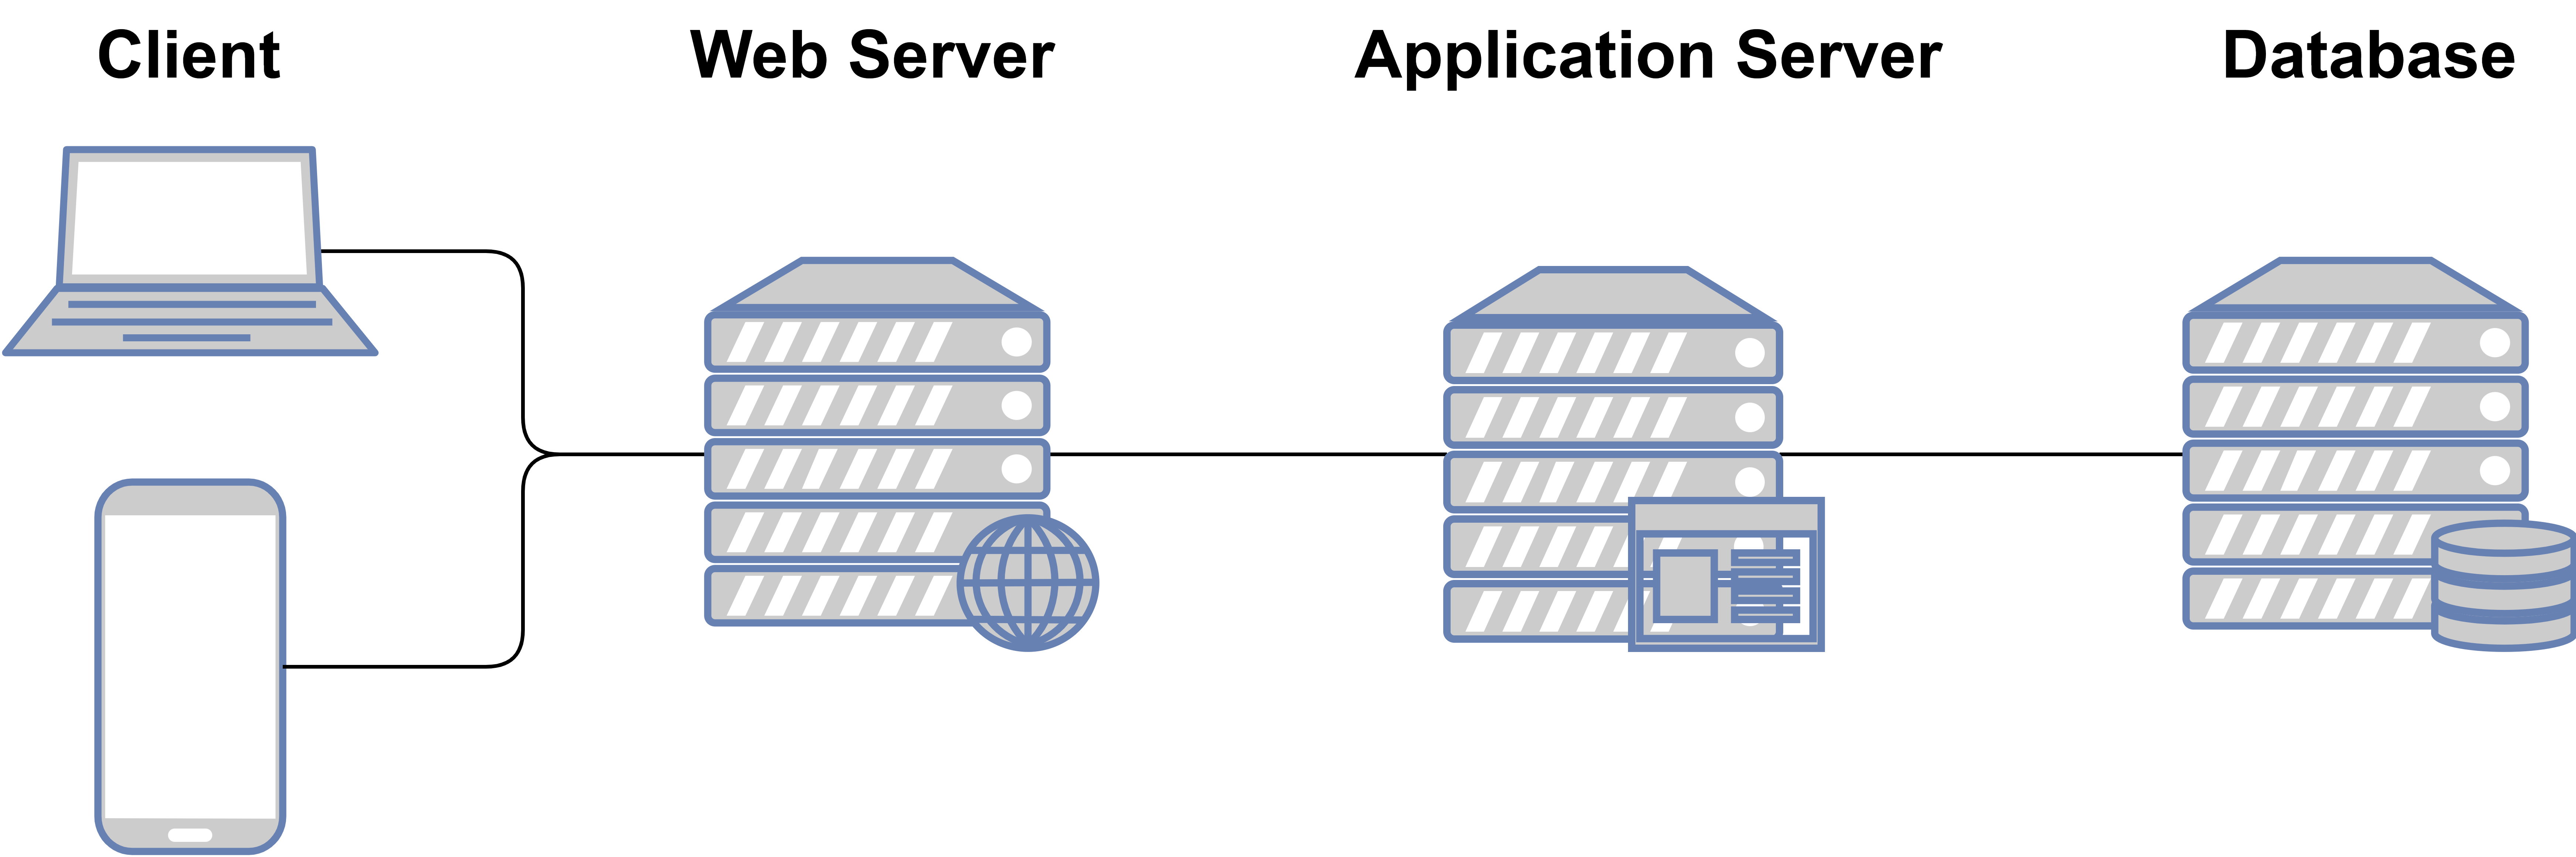
\includegraphics[scale=0.80, center]{assets/3-tier-architecture.png}
        \caption{Three Tier Architecture}
        \label{fig: three_tier_architecture}
    \end{figure}
\end{center}

The system is an application distributed across multiple devices and follows the common client-server paradigm.
The architecture is organized in three logical layers:

\begin{itemize}
    \item \textbf{Presentation Layer (P)}: It's responsible for rendering the application's user interface to the client through the Web Server. It's expressed by a GUI designed to enable the user to interact with the application efficiently.
    \item \textbf{Application Layer (A)}: It's responsible for the business logic of the application. It receives requests from the Presentation Layer, processes them, and then sends back the results to be displayed.
    \item \textbf{Data Layer(D)}: It's in charge of the access to data sources, it provides data through the database and direct it to the other layers. It's also necessary in order to grant a high level of abstraction from the database for an easy to use model.
\end{itemize}

\newpage
\begin{center}
    \begin{figure}[H]
        \includegraphics[scale=0.53, center]{assets/high_level_architecture.png}
        \caption{High Level Architecture}
        \label{fig: high_level_architecture}
    \end{figure}
\end{center}

The system's architecture, as shown in \ref{fig:high_level_architecture}, is composed by a DMZ, that includes the Web and the Mail Server in order to prevent a direct access to the internal system and improve the overall security, and firewalls that divide each newtwork segment.
To reduce computation client side a thin client is used, which allows all the heavy operations to be performed at server side. The Web Server handles the HTTP requests by the users and directs them to the Application Server, while also managing the GoogleMaps API. 
The Application Server communicates with the Database Server and elaborates data following its business logic. The Application server also handles external APIs and services, such as GoogleCalendarAPI, CarAPI, and the exetrnal CPMSs and eMSPs systems.
The Apllication Server's CPMS subsystem will also communicate with its Charging Stations and their relative sockets through the OCPP API, and with the external DSOs through their proprietary API.
The Email Server will manage all the e-mail notification by communicating with the Application Server, The database server is responsible for storing and managing the data that is used by the application. It receives requests for data from the application logic tier, retrieves the requested data from the database, and returns the data to the application logic tier.

\subsection{Component view}
\subsubsection*{General Component View}
\begin{center}
    \begin{figure}[H]
        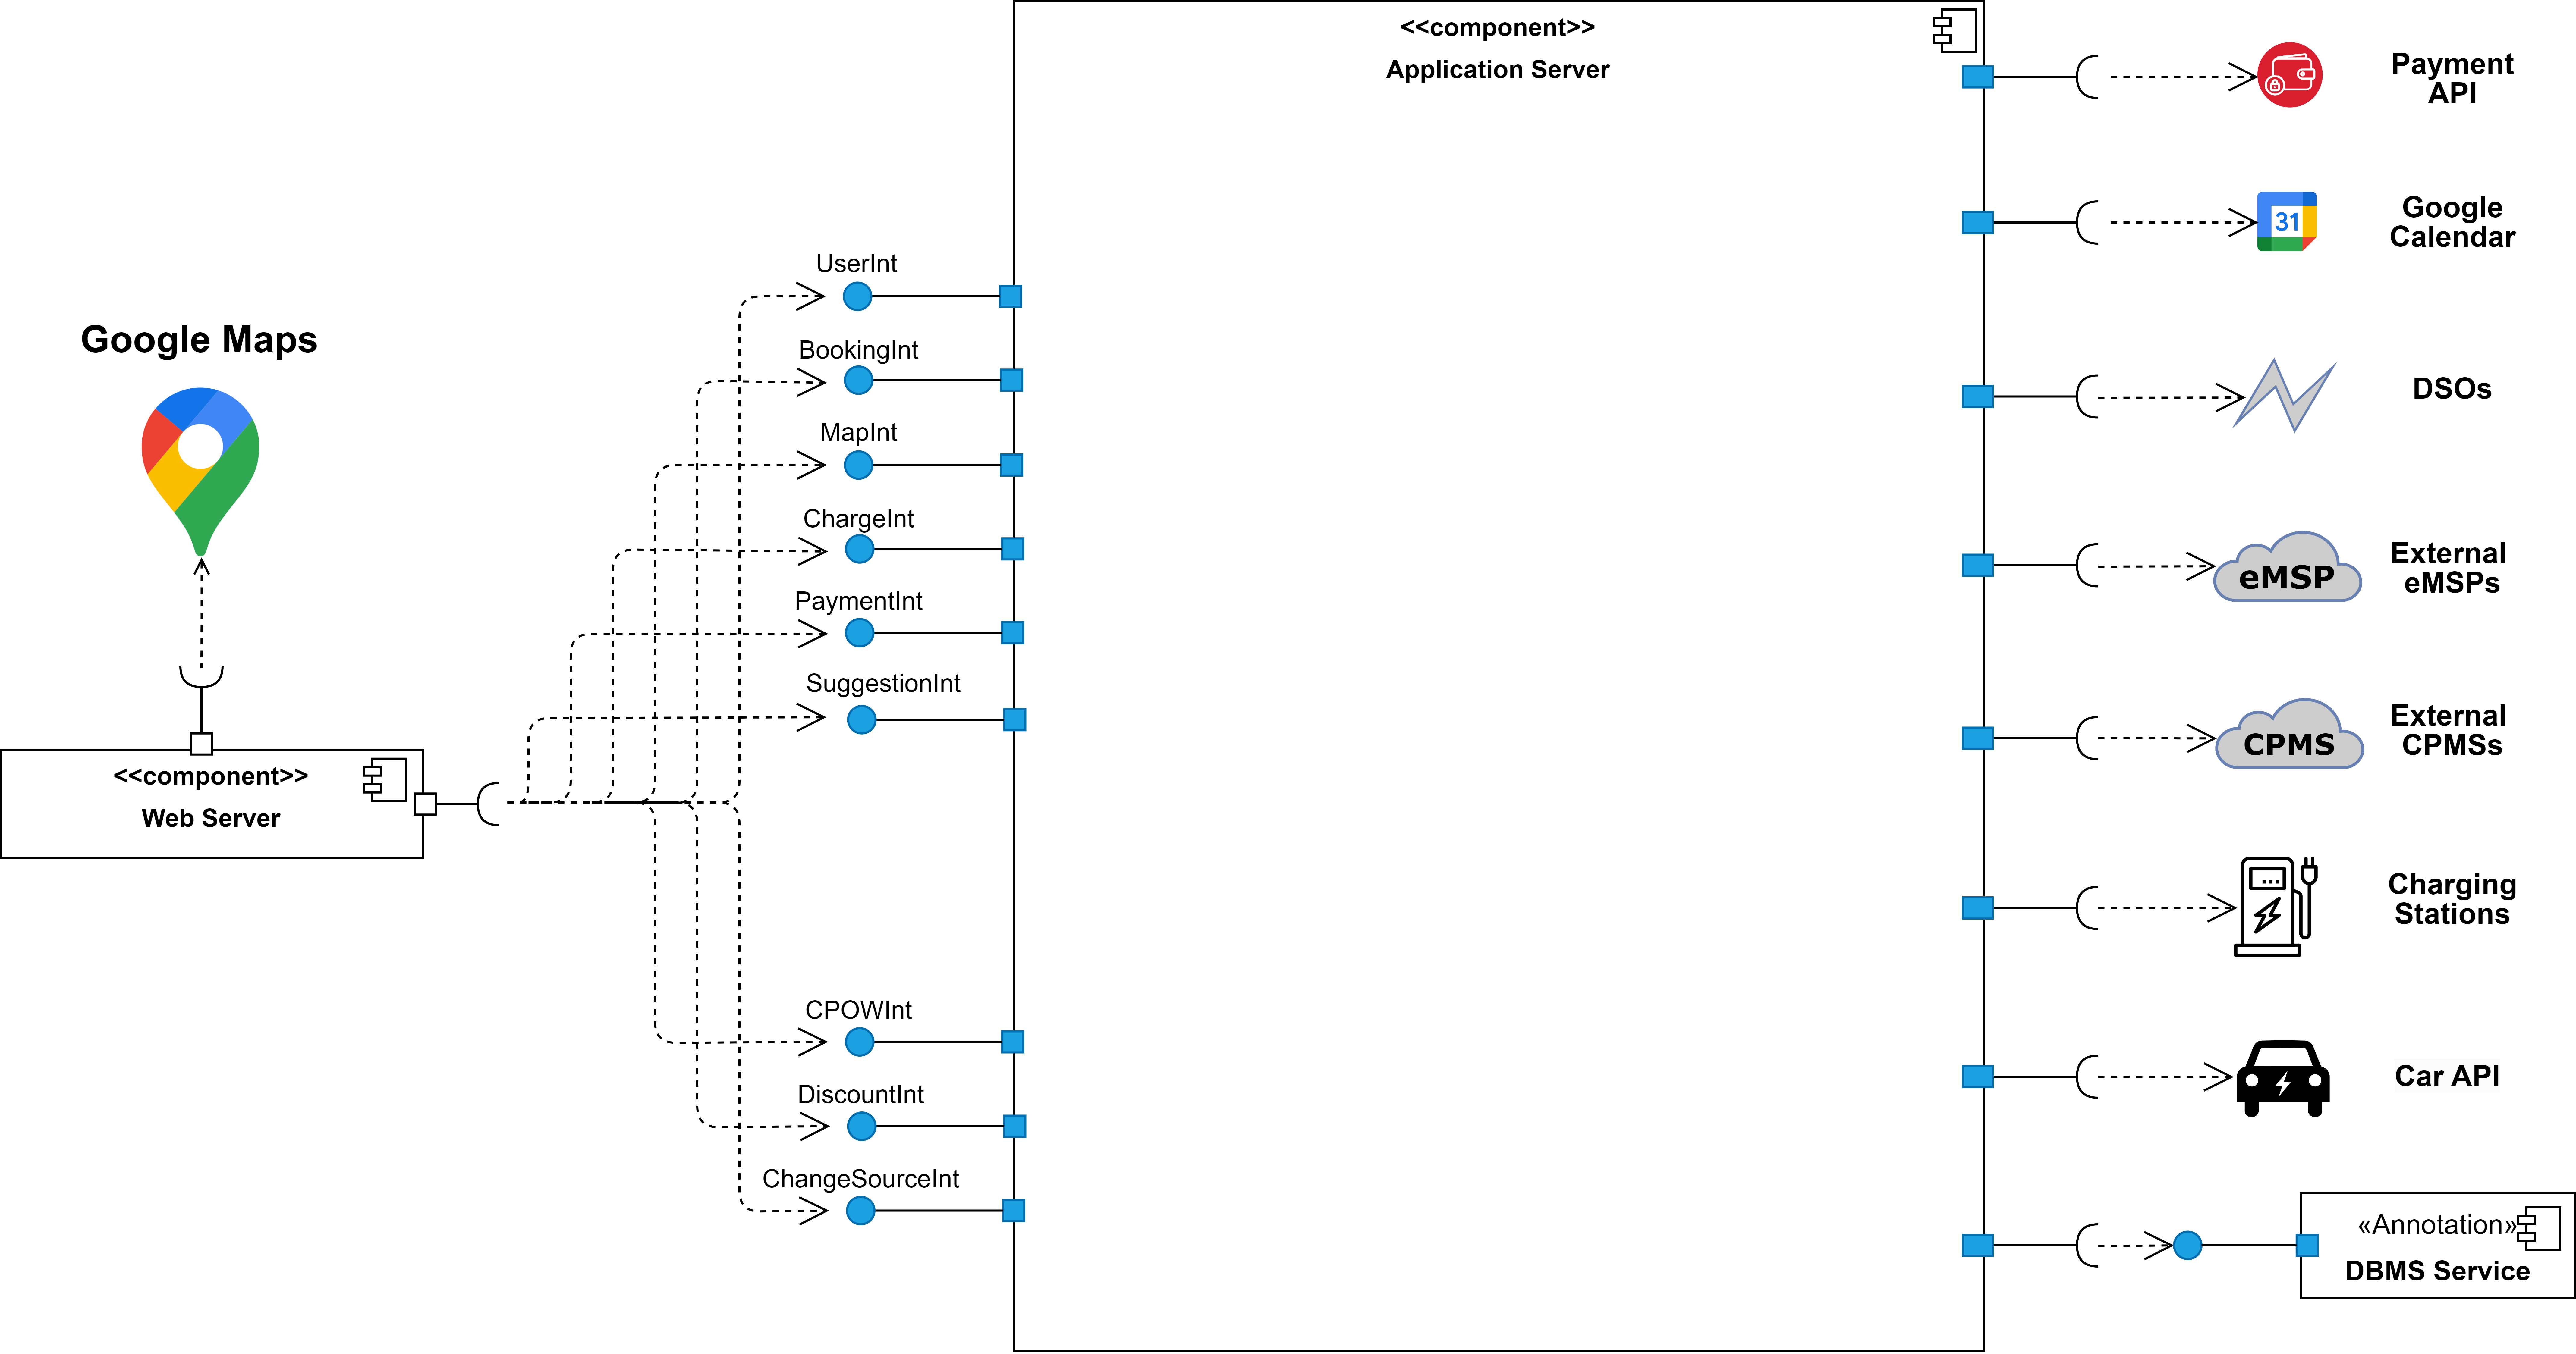
\includegraphics[scale=0.65, center]{assets/general_component_diagram.png}
        \caption{General Component Diagram}
        \label{fig: general_component_view}
    \end{figure}
\end{center}

This image gives a high level representation of the components of the system.
In the scheme the application server is represented by an empty box, since a complete description will be provided in the next section. On the left the interfaces between the web server and the application server are shown; these basically represent the main functionalities requested by the client applications. On the opposite site the external interfaces are presented, among which there are the interfaces to other CPMSs and to the charging stations. Additionally, there's also the DBMS iterface, which manages the DBMS service and handles all communications between the Applicantion server and the Database server. 

\subsubsection*{Application Server Component View}
\begin{center}
    \begin{figure}[H]
        \includegraphics[scale=0.33, center]{assets/application-server-component-diagram.png}
        \caption{Application Server Component Diagram}
        \label{fig: application_server_component_view}
    \end{figure}
\end{center}

The following component diagram gives a detailed view of the Application Server. It shows the internal structure and the interaction between the components.
External elements in the diagram are represented in a simplified way.
\\
\textbf{eMSP subsystem}
\begin{itemize}
    \item \textbf{AccountManager}: Handles all the basic requests that a client can make. Among those the \textit{AuthenticationService} manages the authentication process (log in, log out, sign up). All the specific functionalities are then provided once the user logs in.
    \item \textbf{eMSP\_UserManager}: It manages all the services available to the eSMP subsystem's users. Various services are then handled by other components, for example the \textit{BookingService} is handled by the \textit{BookingManager}, which communicates through the OCPI component with the CPMSs. Most services also communicate with the Database through an interface.
    \item \textbf{BookingManager}: It handles all the booking requests made by the clients and is responsible for sending the requests to the CPMS through the OCPI component.
    \item \textbf{ChargingProcessManager}: This component manages the charging process service of the user's car, in particular it provides updated informations about the charging status while interacting with the OCPI component to retrive informations and also managing the start and stop charging functions.
    \item \textbf{ChargingStationManager}: This component  handles the Charging Stations general informations and status to be displayed through the \textit{InteractiveMapService}. To do so it interacts with the OCPI component to retrive all the info from the CPMSs.
    \item \textbf{PaymentManager}: It manages the paymentService. It interacts with the external component \textit{Payment}.
    \item \textbf{SuggestionManager}: It handles the service that generates suggestions for the users on when to charge the car. In order to do that it communicates with the \textit{EVmanager} and with the \textit{CalendarManager} to get all the informations needed to formulate suggestions, in particular the user's schedule and the car battery status.
    \item \textbf{CalendarManager}: This component manages the information relative to the user's schedule for the \textit{SuggestionService}. To do so it interfaces with the external component \textit{Calendar}.
    \item \textbf{EVManager}: This component handles the information relative to the user cars' battery status for the \textit{SuggestionService}. To do so it interfaces with the external component \textit{CarAPI}.
\end{itemize}

\subsubsection*{Web Server Component View}
Regarding the Web Server the main components are:
\begin{itemize}
    \item \textbf{first component}: description of component.
\end{itemize}

\newpage

\subsection{Deployment view}
\begin{center}
    \begin{figure}[H]
        
\includegraphics[scale=0.45, center]{assets/placeholder.png}
        \caption{Deployment Diagram}
        \label{fig: deployment_diagram}
    \end{figure}
\end{center}

The deployment diagram in \textit{Figure (\ref{fig: deployment_diagram})} shows the most important components necessary for the correct behaviour of the system.
The devices shown in the diagram are:
\begin{itemize}
    \item \textbf{first device/component}: description of device (e.g. pc or Smartphone, firewall, load balancer, web server, app server, database server...).
\end{itemize}
\newpage

\subsection{Runtime view}

In this section we list some relevant use cases of the system, represented through sequence diagrams. 
In some diagrams, interactions like the login phase, returning to home page or retrieve the same kind of data were omitted for the sake of clarity.

\newpage
\underline{\textbf{Shared diagrams}}\\
\textbf{Sign Up}
\begin{center}
    \begin{figure}[H]
        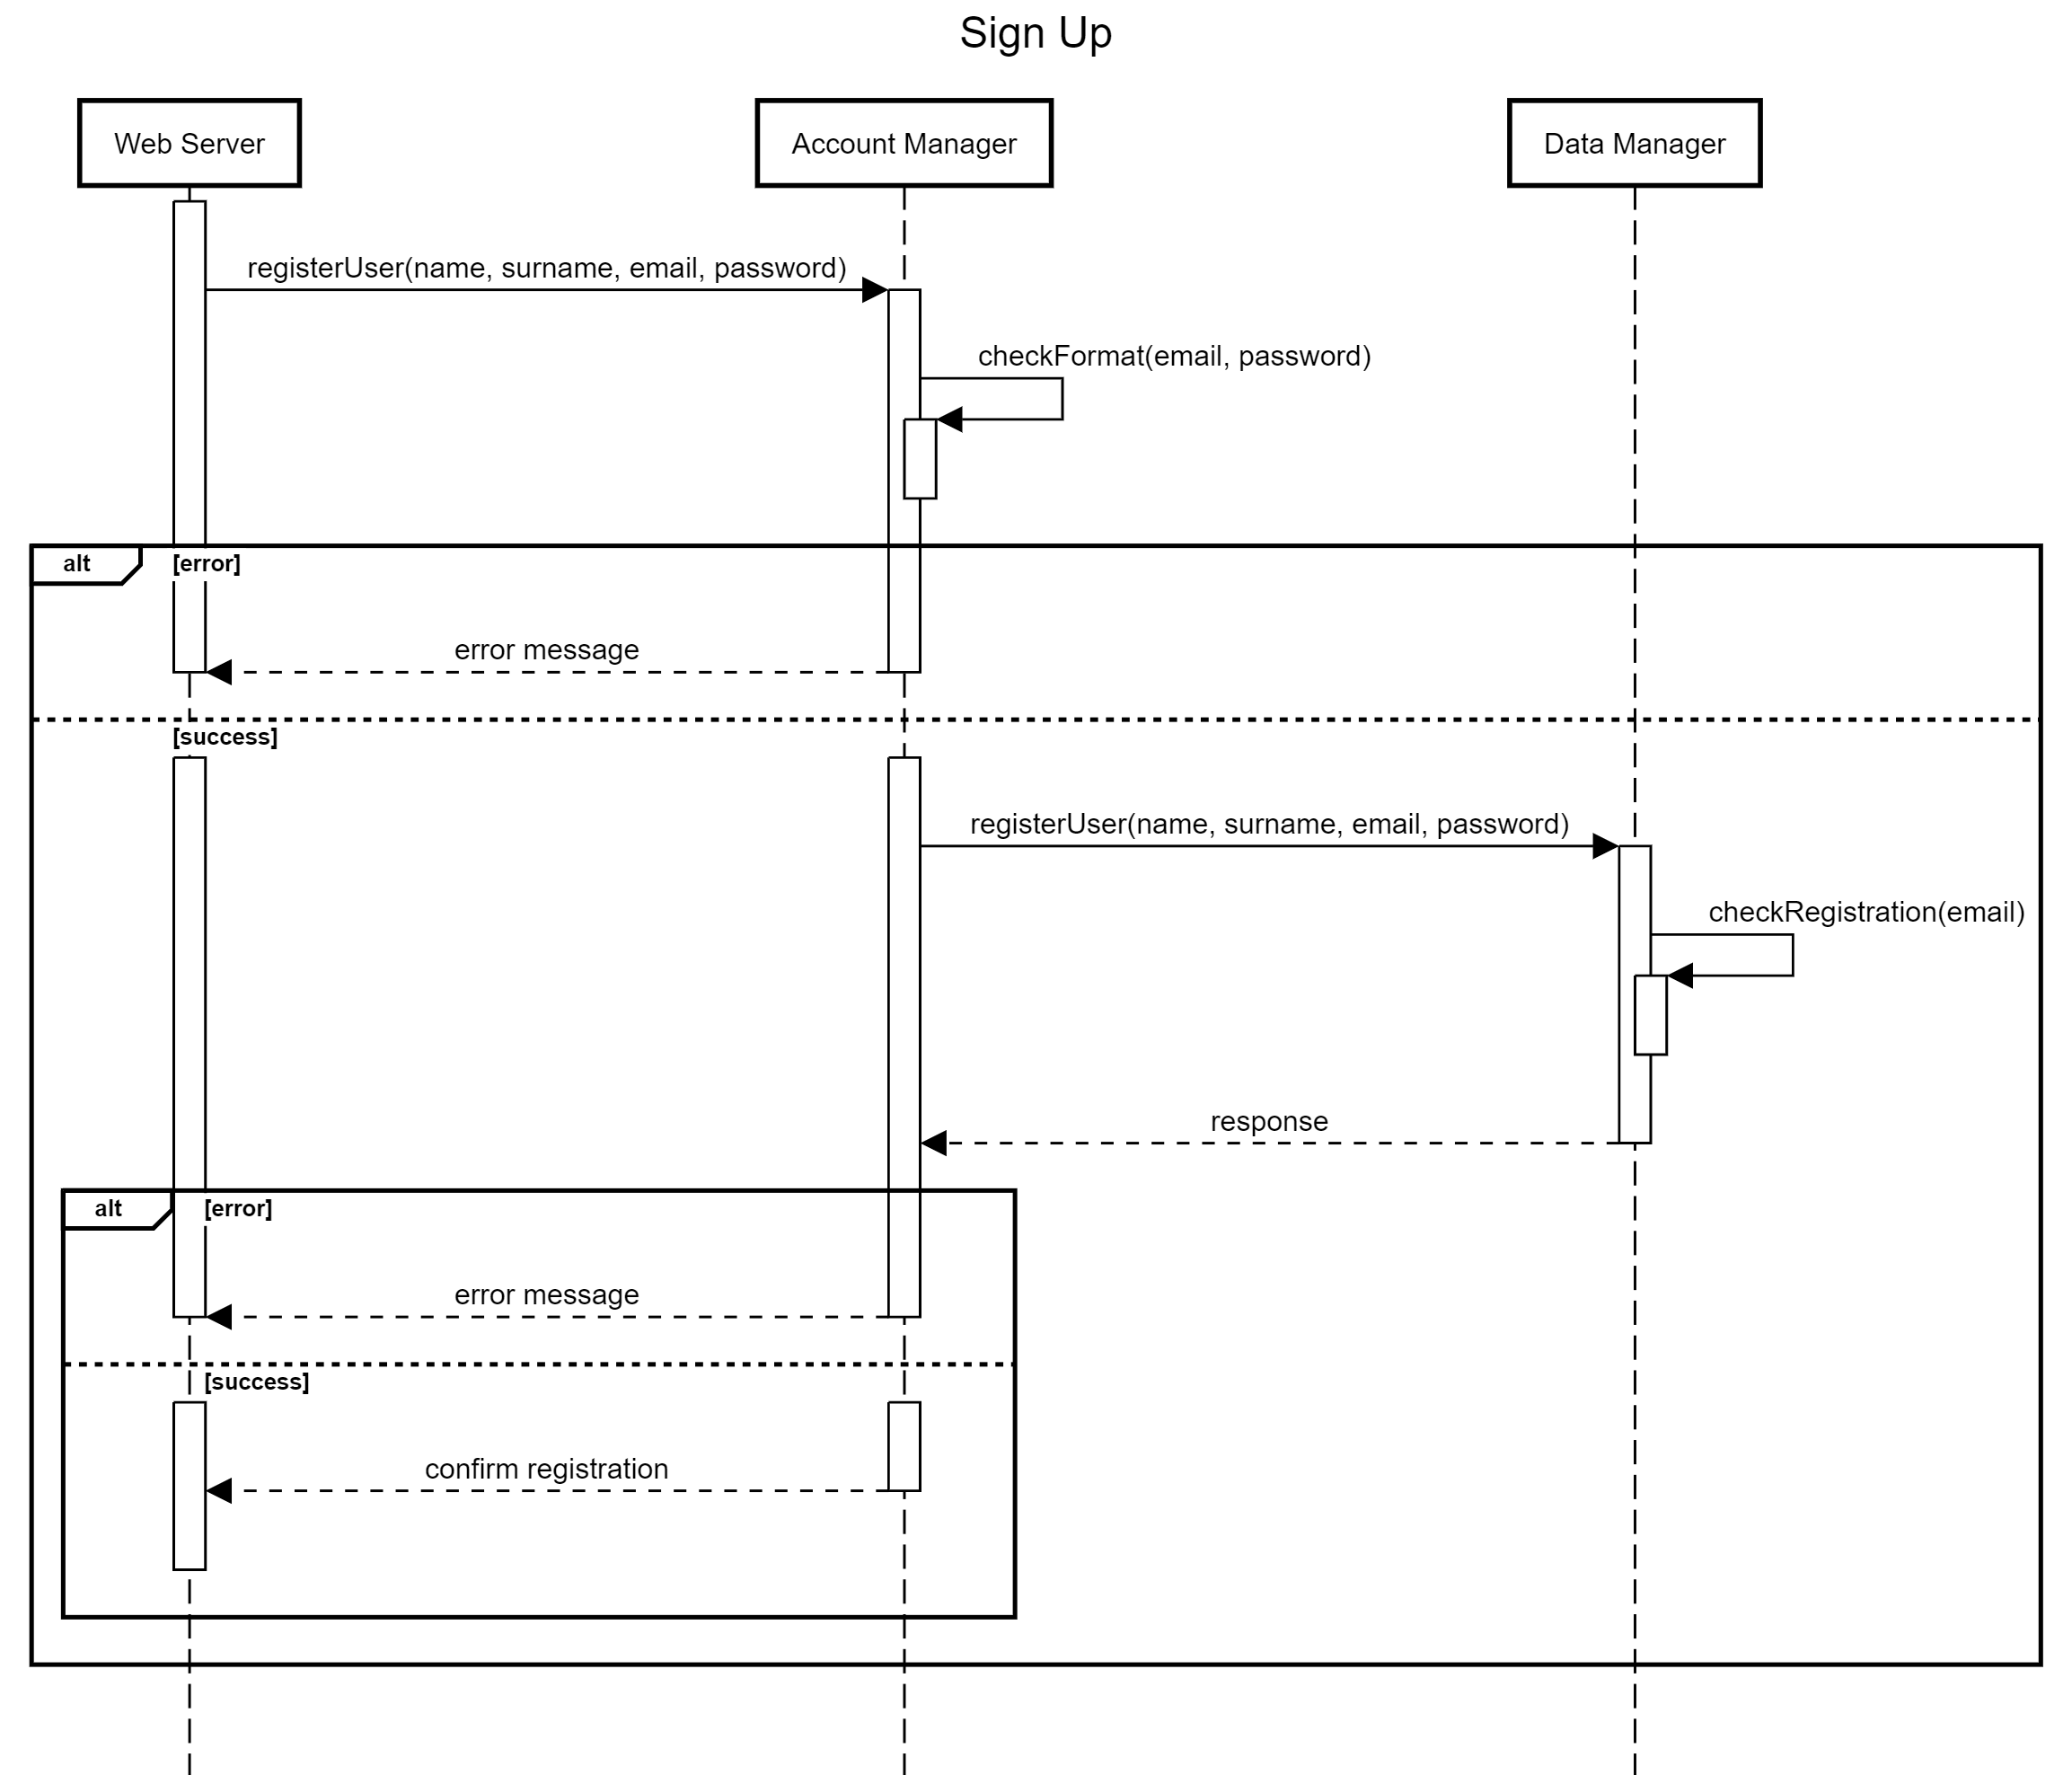
\includegraphics[scale=0.15, center]{assets/sequenceDiagrams/shared signup.png}
        \caption{Sign Up}
        \label{fig:signup}
    \end{figure}
\end{center}
The Sign-up phase consists in the user action of inserting their personal data in the sign-up fields, then the system checks if the email (unique key in the database) is already present in the database.
If it's not, the user can sign up and use the system functionalities available for that particular type of account depending if he's registering through the eMSP or the CPMS.

\newpage

\textbf{Log In}
\begin{center}
    \begin{figure}[H]
        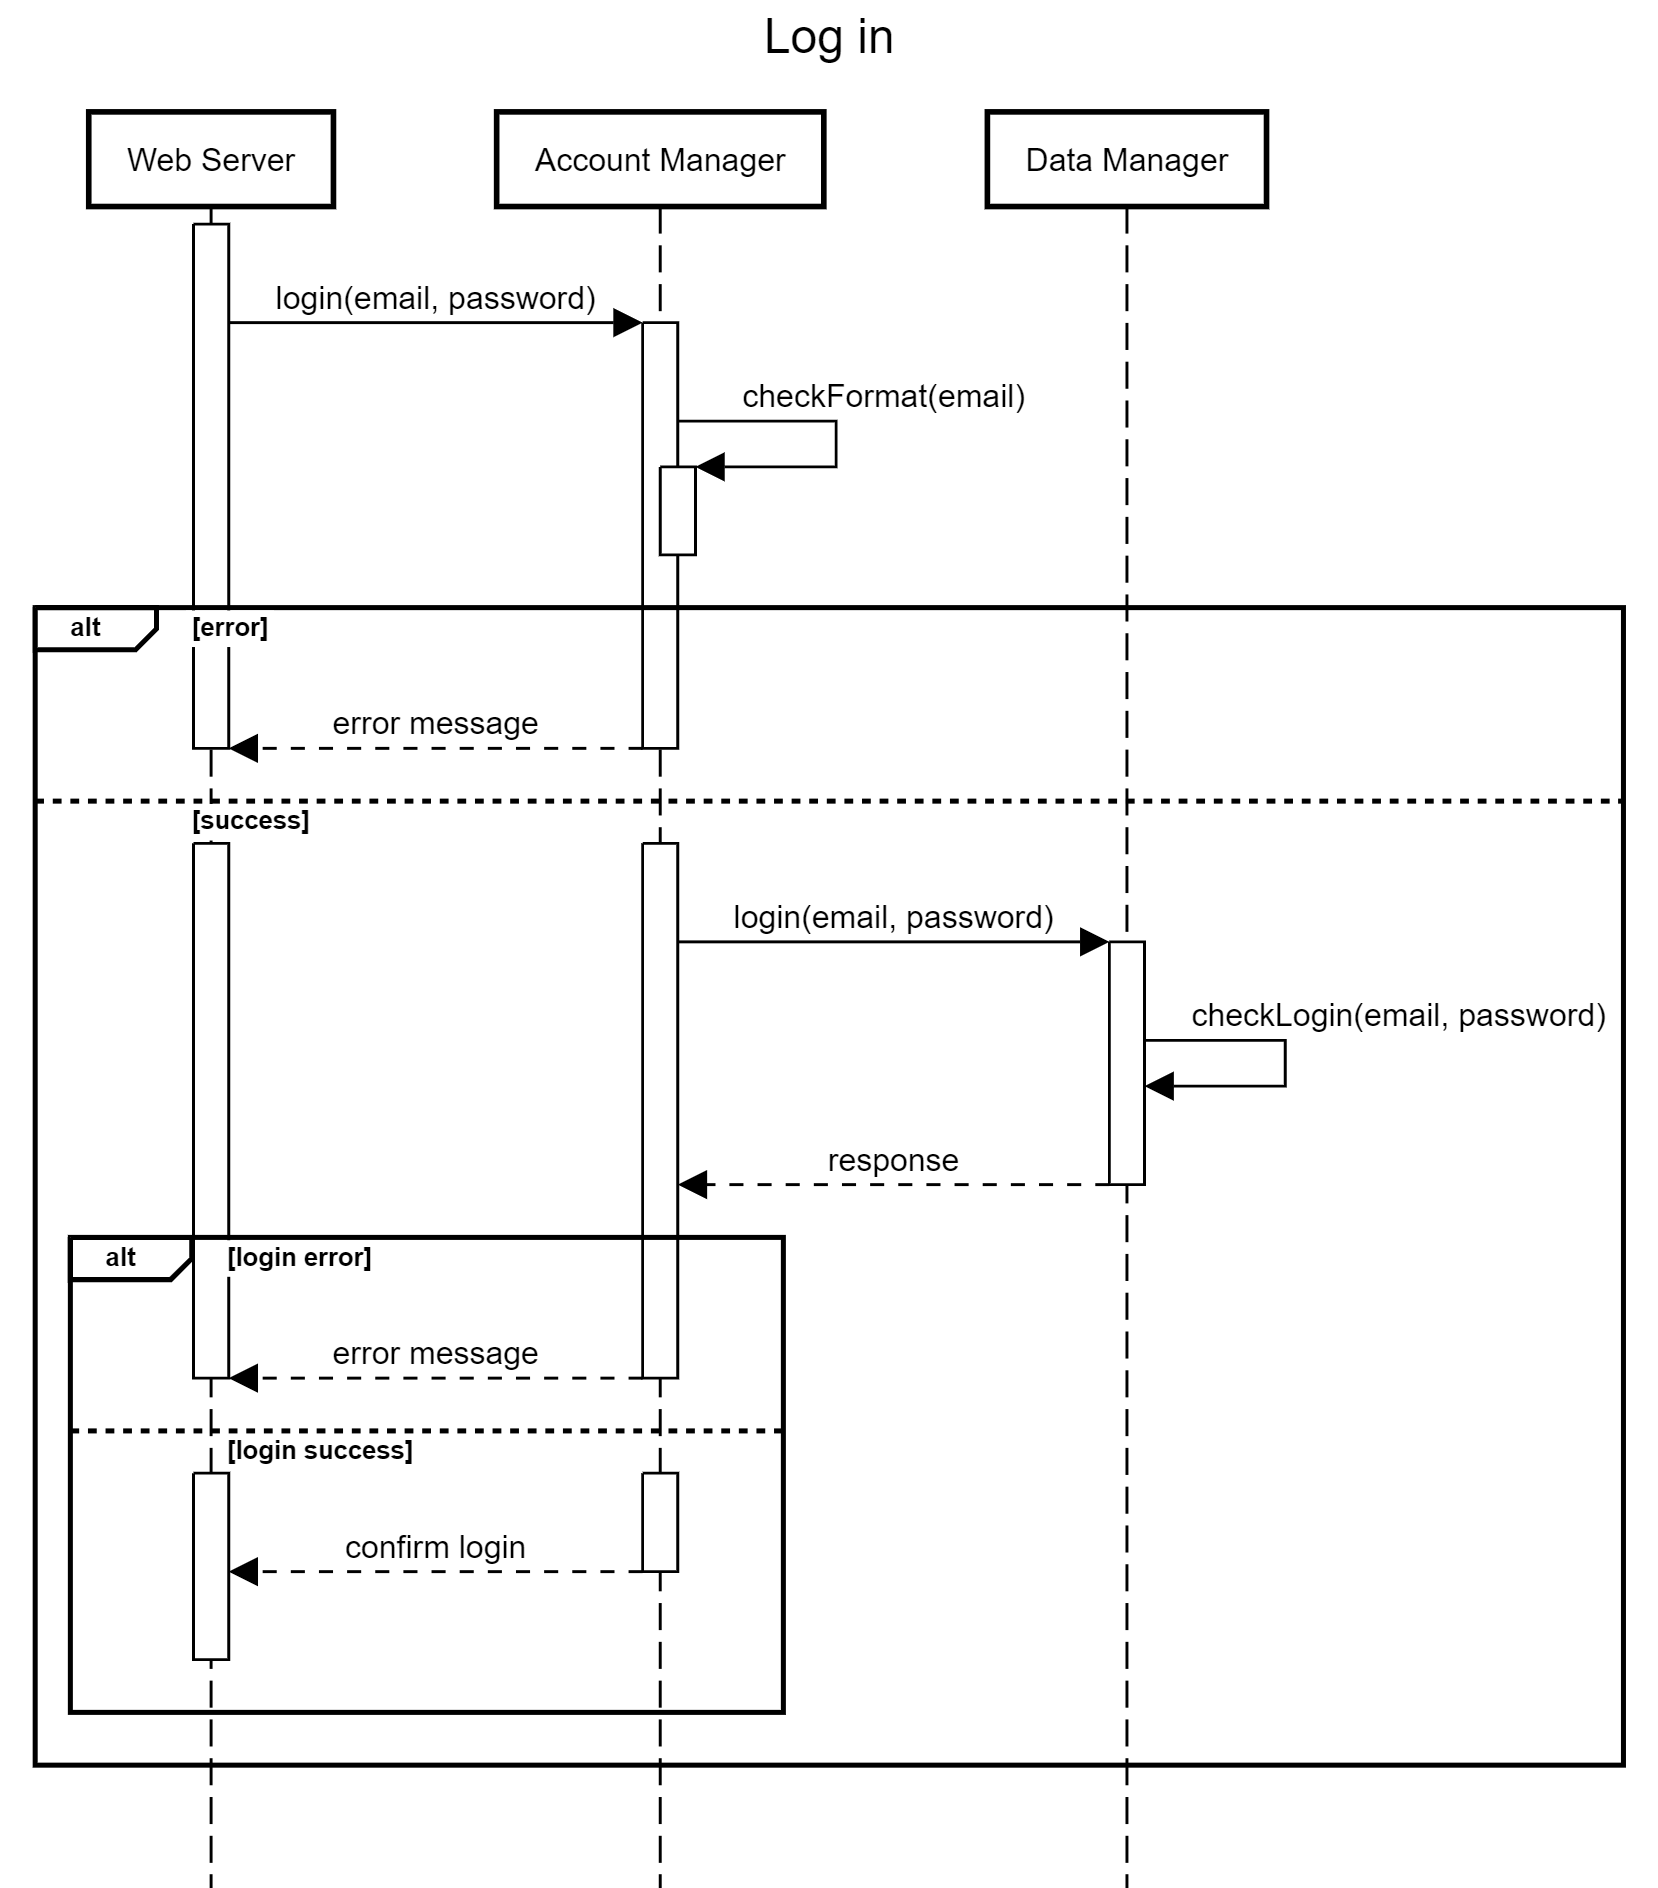
\includegraphics[scale=0.2, center]{assets/sequenceDiagrams/shared login.png}
        \caption{Log In}
        \label{fig: login}
    \end{figure}
\end{center}

The Log In phase consists in the user action of inserting their email (unique key in the database) and password in the login fields, then the system checks if the pair corresponds to a user entry in the database.
In case of success, the user can log-in and use the system functionalities available for that particular type of account depending if he's logging in through the eMSP or the CPMS.

\newpage
\underline{\textbf{User diagrams}}\\

\textbf{View Nearby Stations}
\begin{center}
    \begin{figure}[H]
        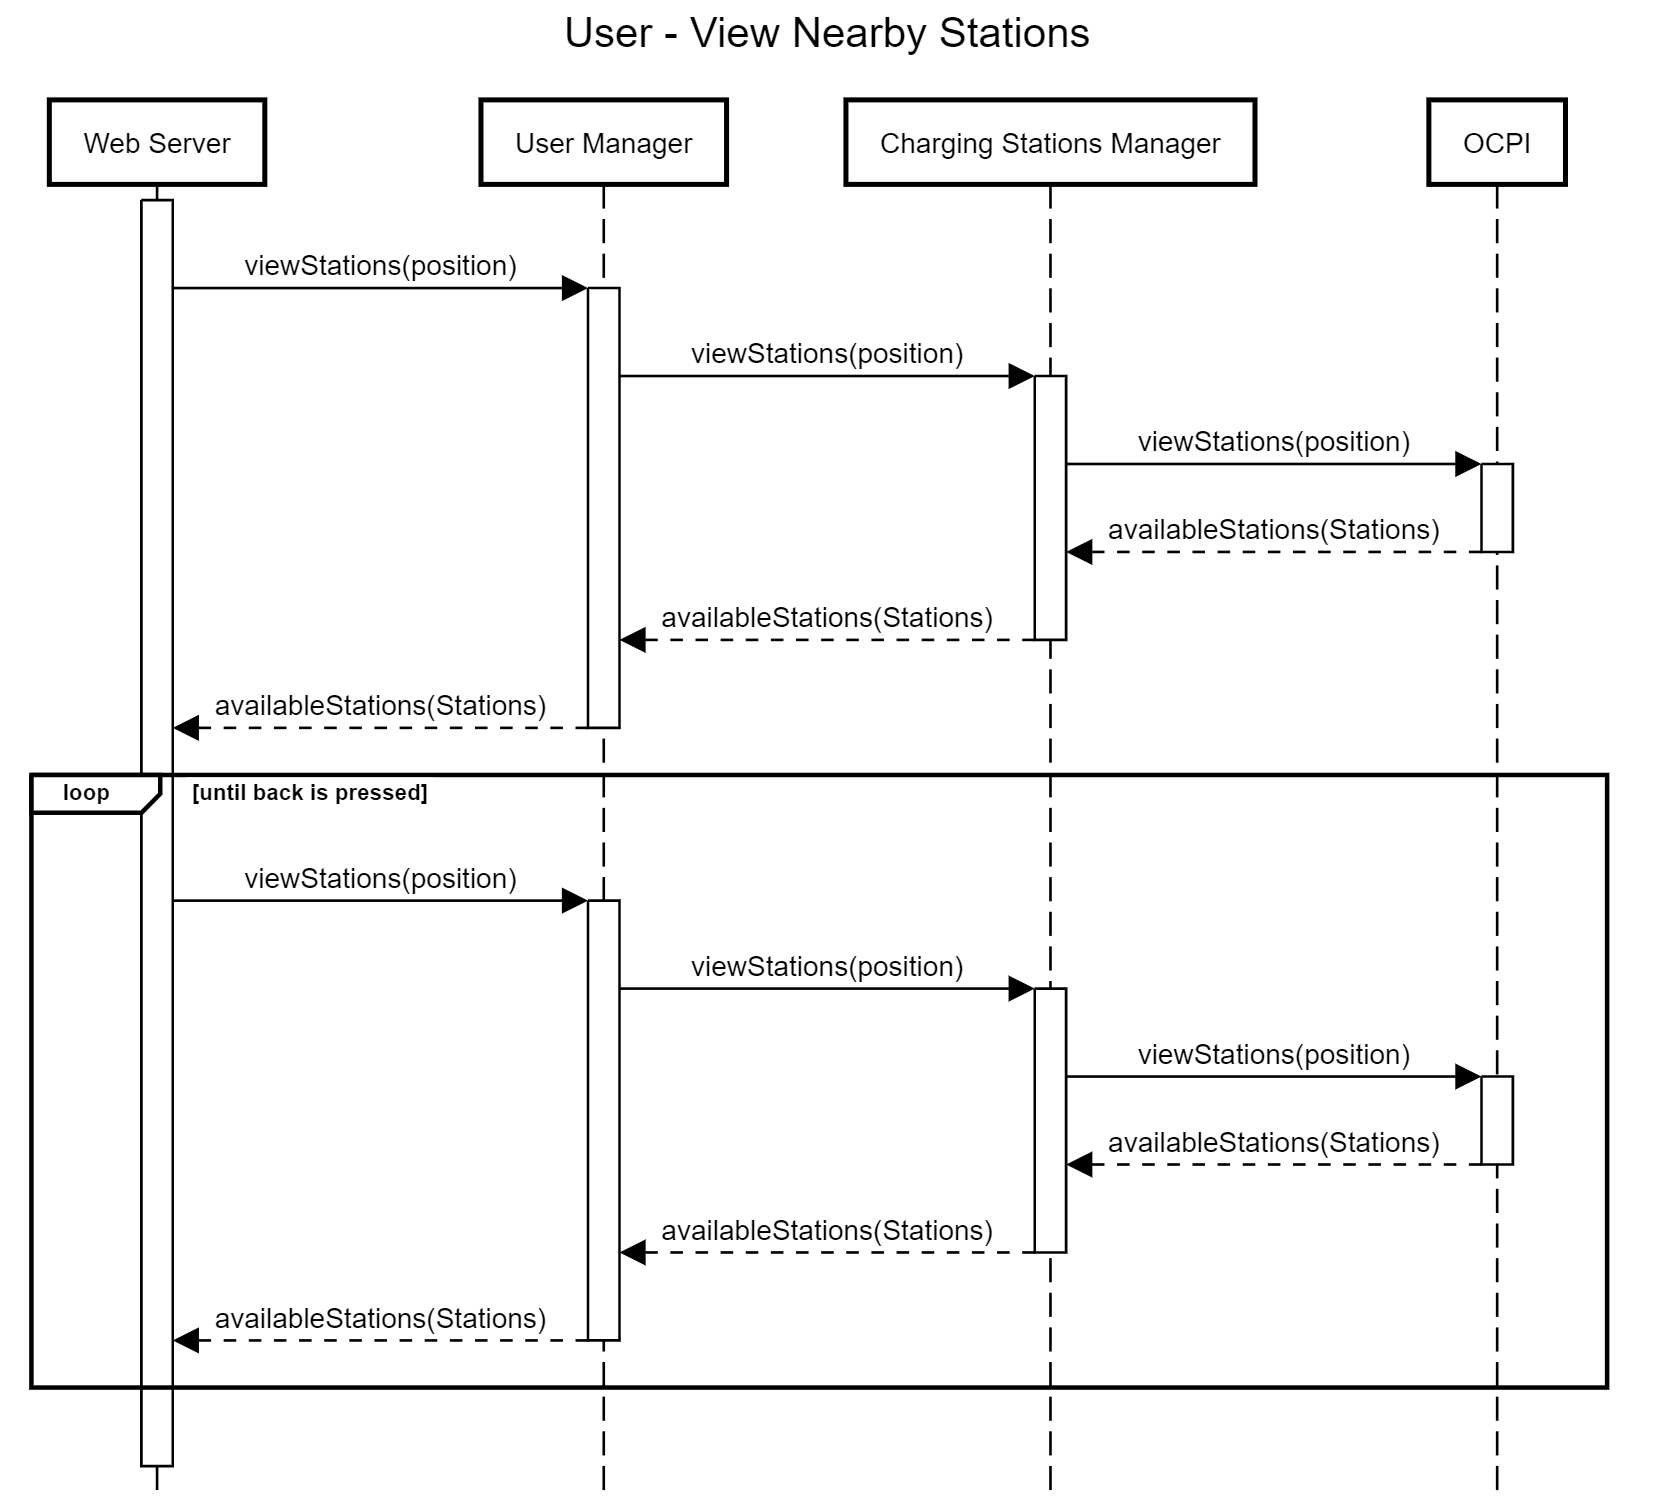
\includegraphics[scale=0.15, center]{assets/sequenceDiagrams/User View Nearby Stations.png}
        \caption{Sign Up}
        \label{View Nearby Stations}
    \end{figure}
\end{center}
The view nearby stations is the process through which the interactive map is updated when the user is inside the webapp. In this diagram it is assumed the user is already on the interactive map part.
Upon detecting the user's movement on the map, the server retrieves the new stations that must be loaded caused by the movement. This process is repeated while the user is navigating on the map, and ends only when the user exits it.

\newpage

\textbf{Delete a Booking}
\begin{center}
    \begin{figure}[H]
        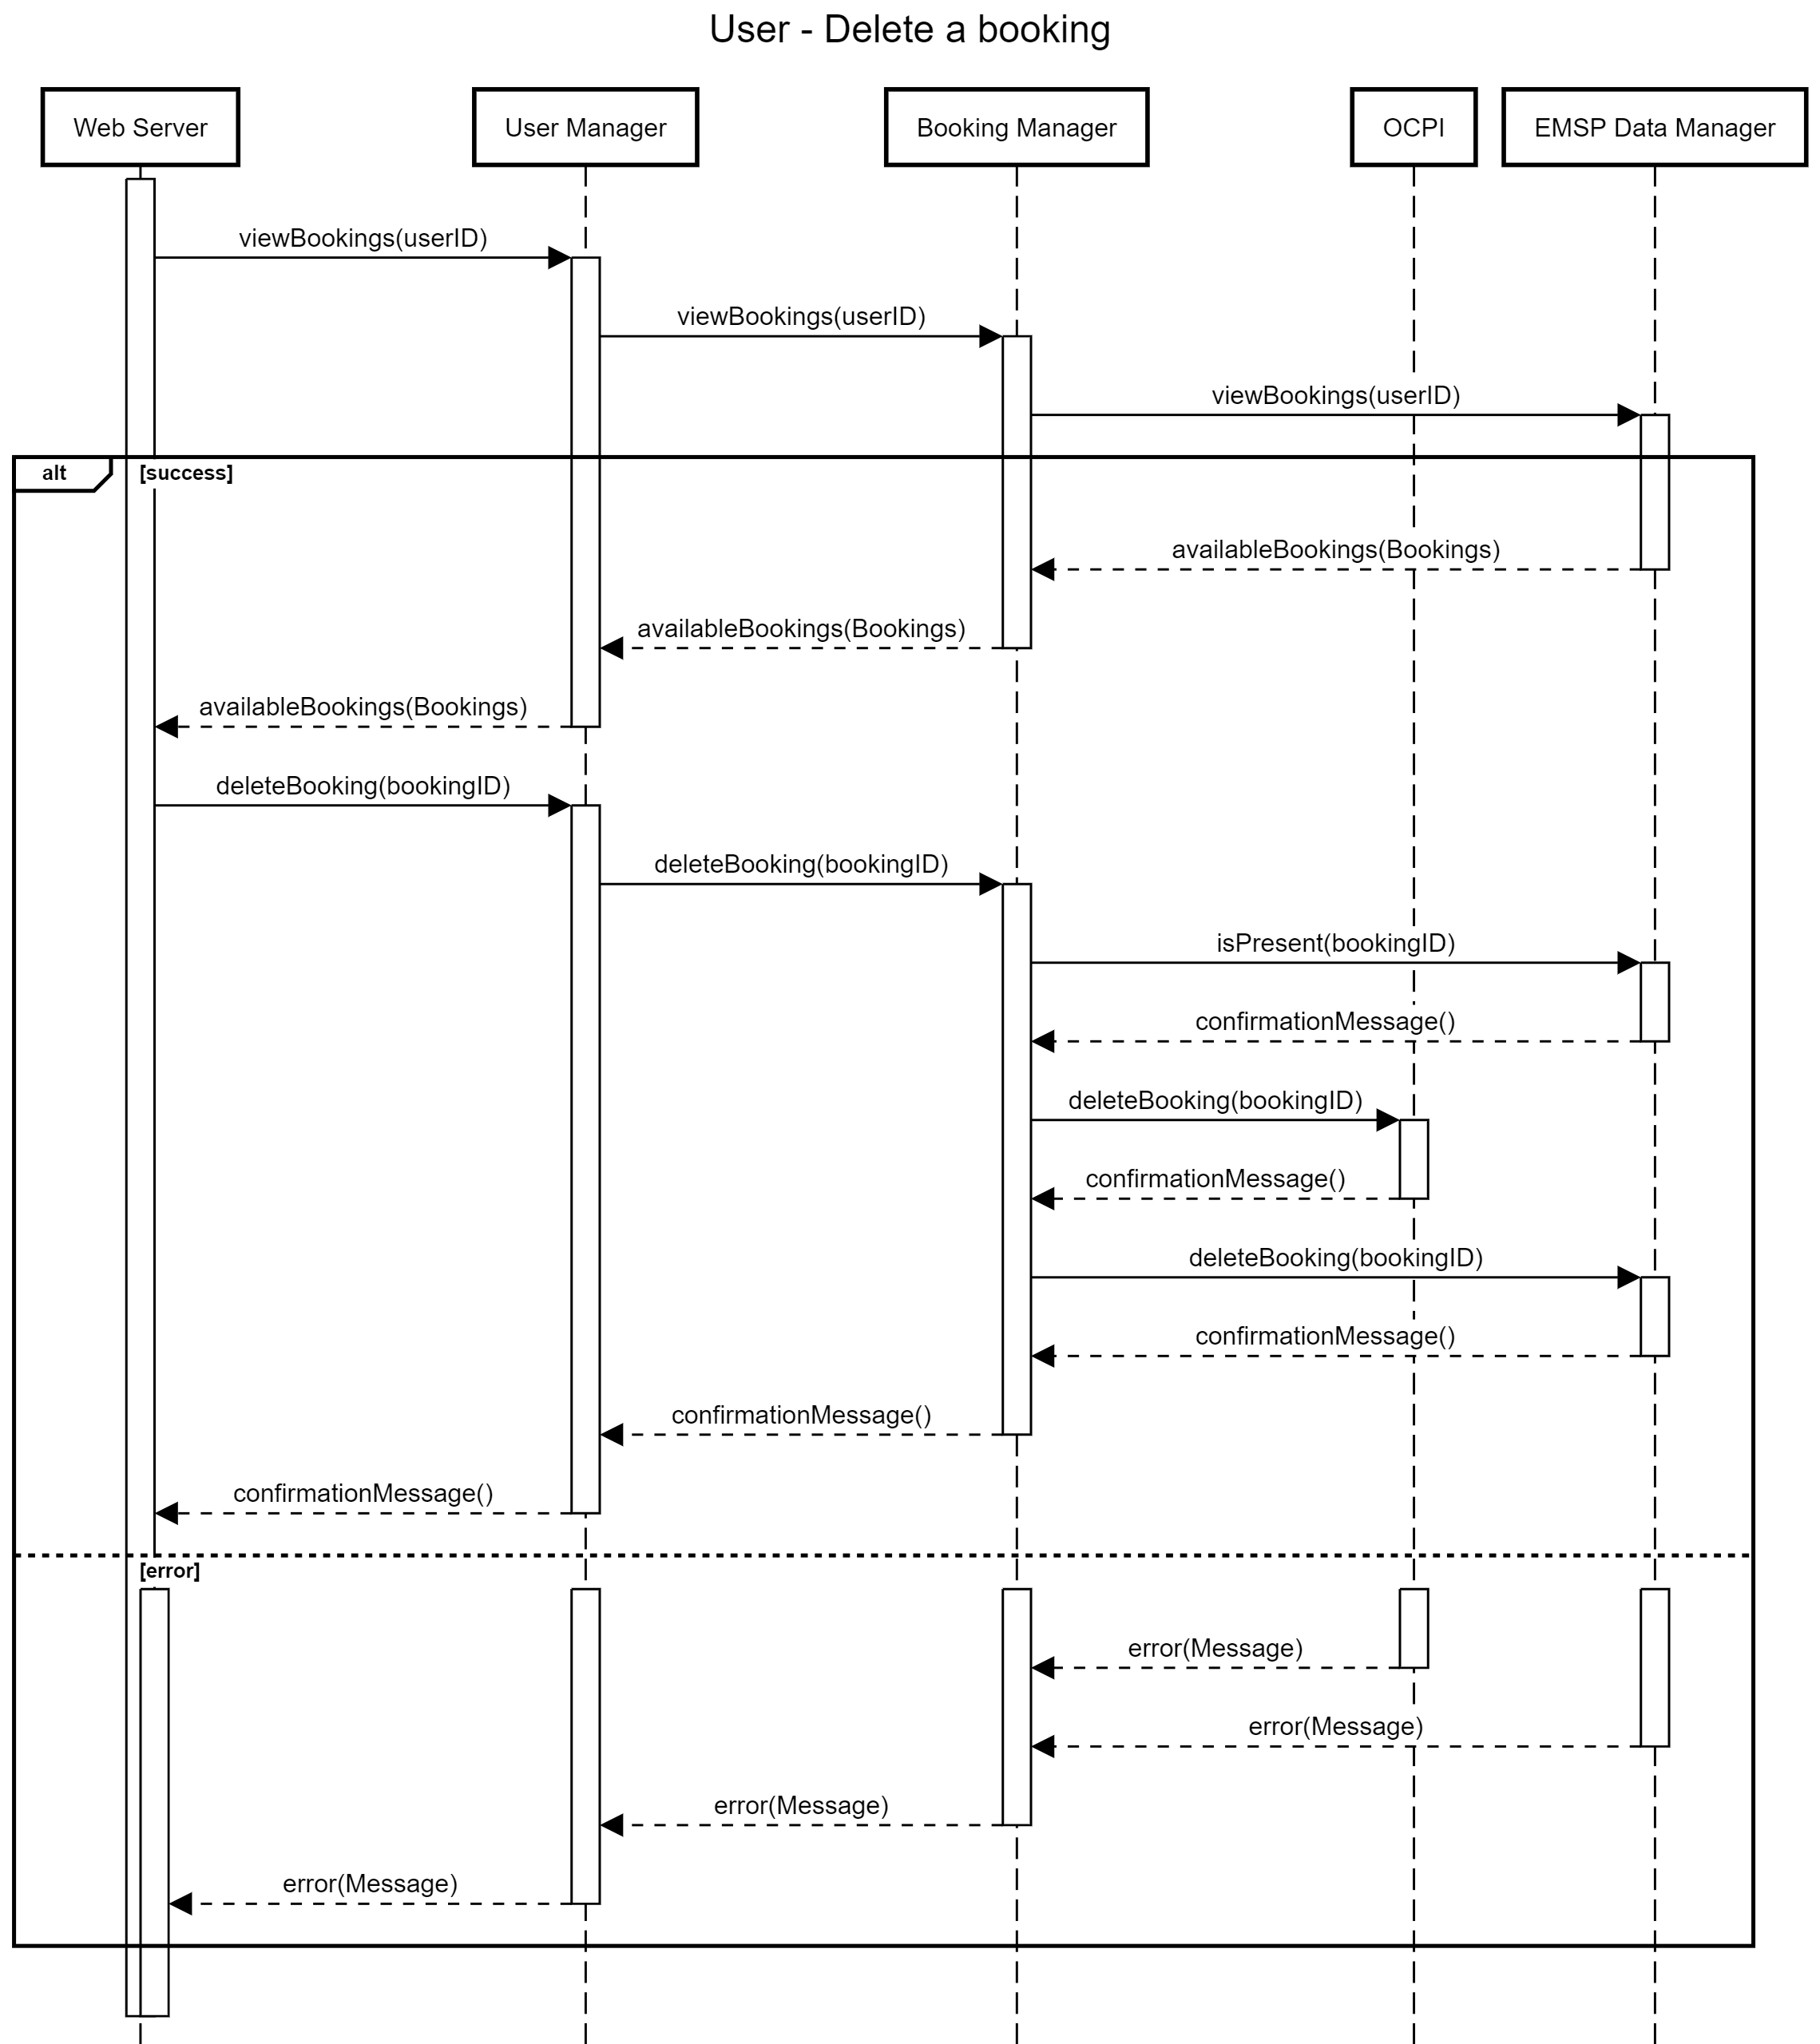
\includegraphics[scale=0.15, center]{assets/sequenceDiagrams/User delete bookings.png}
        \caption{Sign Up}
        \label{Delete Booking}
    \end{figure}
\end{center}
In the first part of the sequence the user is viewing his bookings list and clicks on "Delete" on one of them. The id of said selected booking is then sent to process the deletion request.
Firstly, a check by the Booking Manager is done to assure the bookingID sent is actually present on the database of that user's bookings. If present, the Booking Manager proceeds to firstly delete the booking from the 
interested station(communicating with OCPI) then deleting it from the user's bookings on the database (communicating with eMSP Data Manager again).
 For the sake of readability, all errors are pushed to the end and will be furhter explained here by text. The first error that can happen is caused by the user not having any active bookings.
 The second possible error is caused by the first check in case the bookingID that has to be deleted doesn't exist in the database.
 Lastly, an error could be caused by the requested booking not existing on the OCPI. 

\newpage
\textbf{Make a Booking}
 \begin{center}
    \begin{figure}[H]
        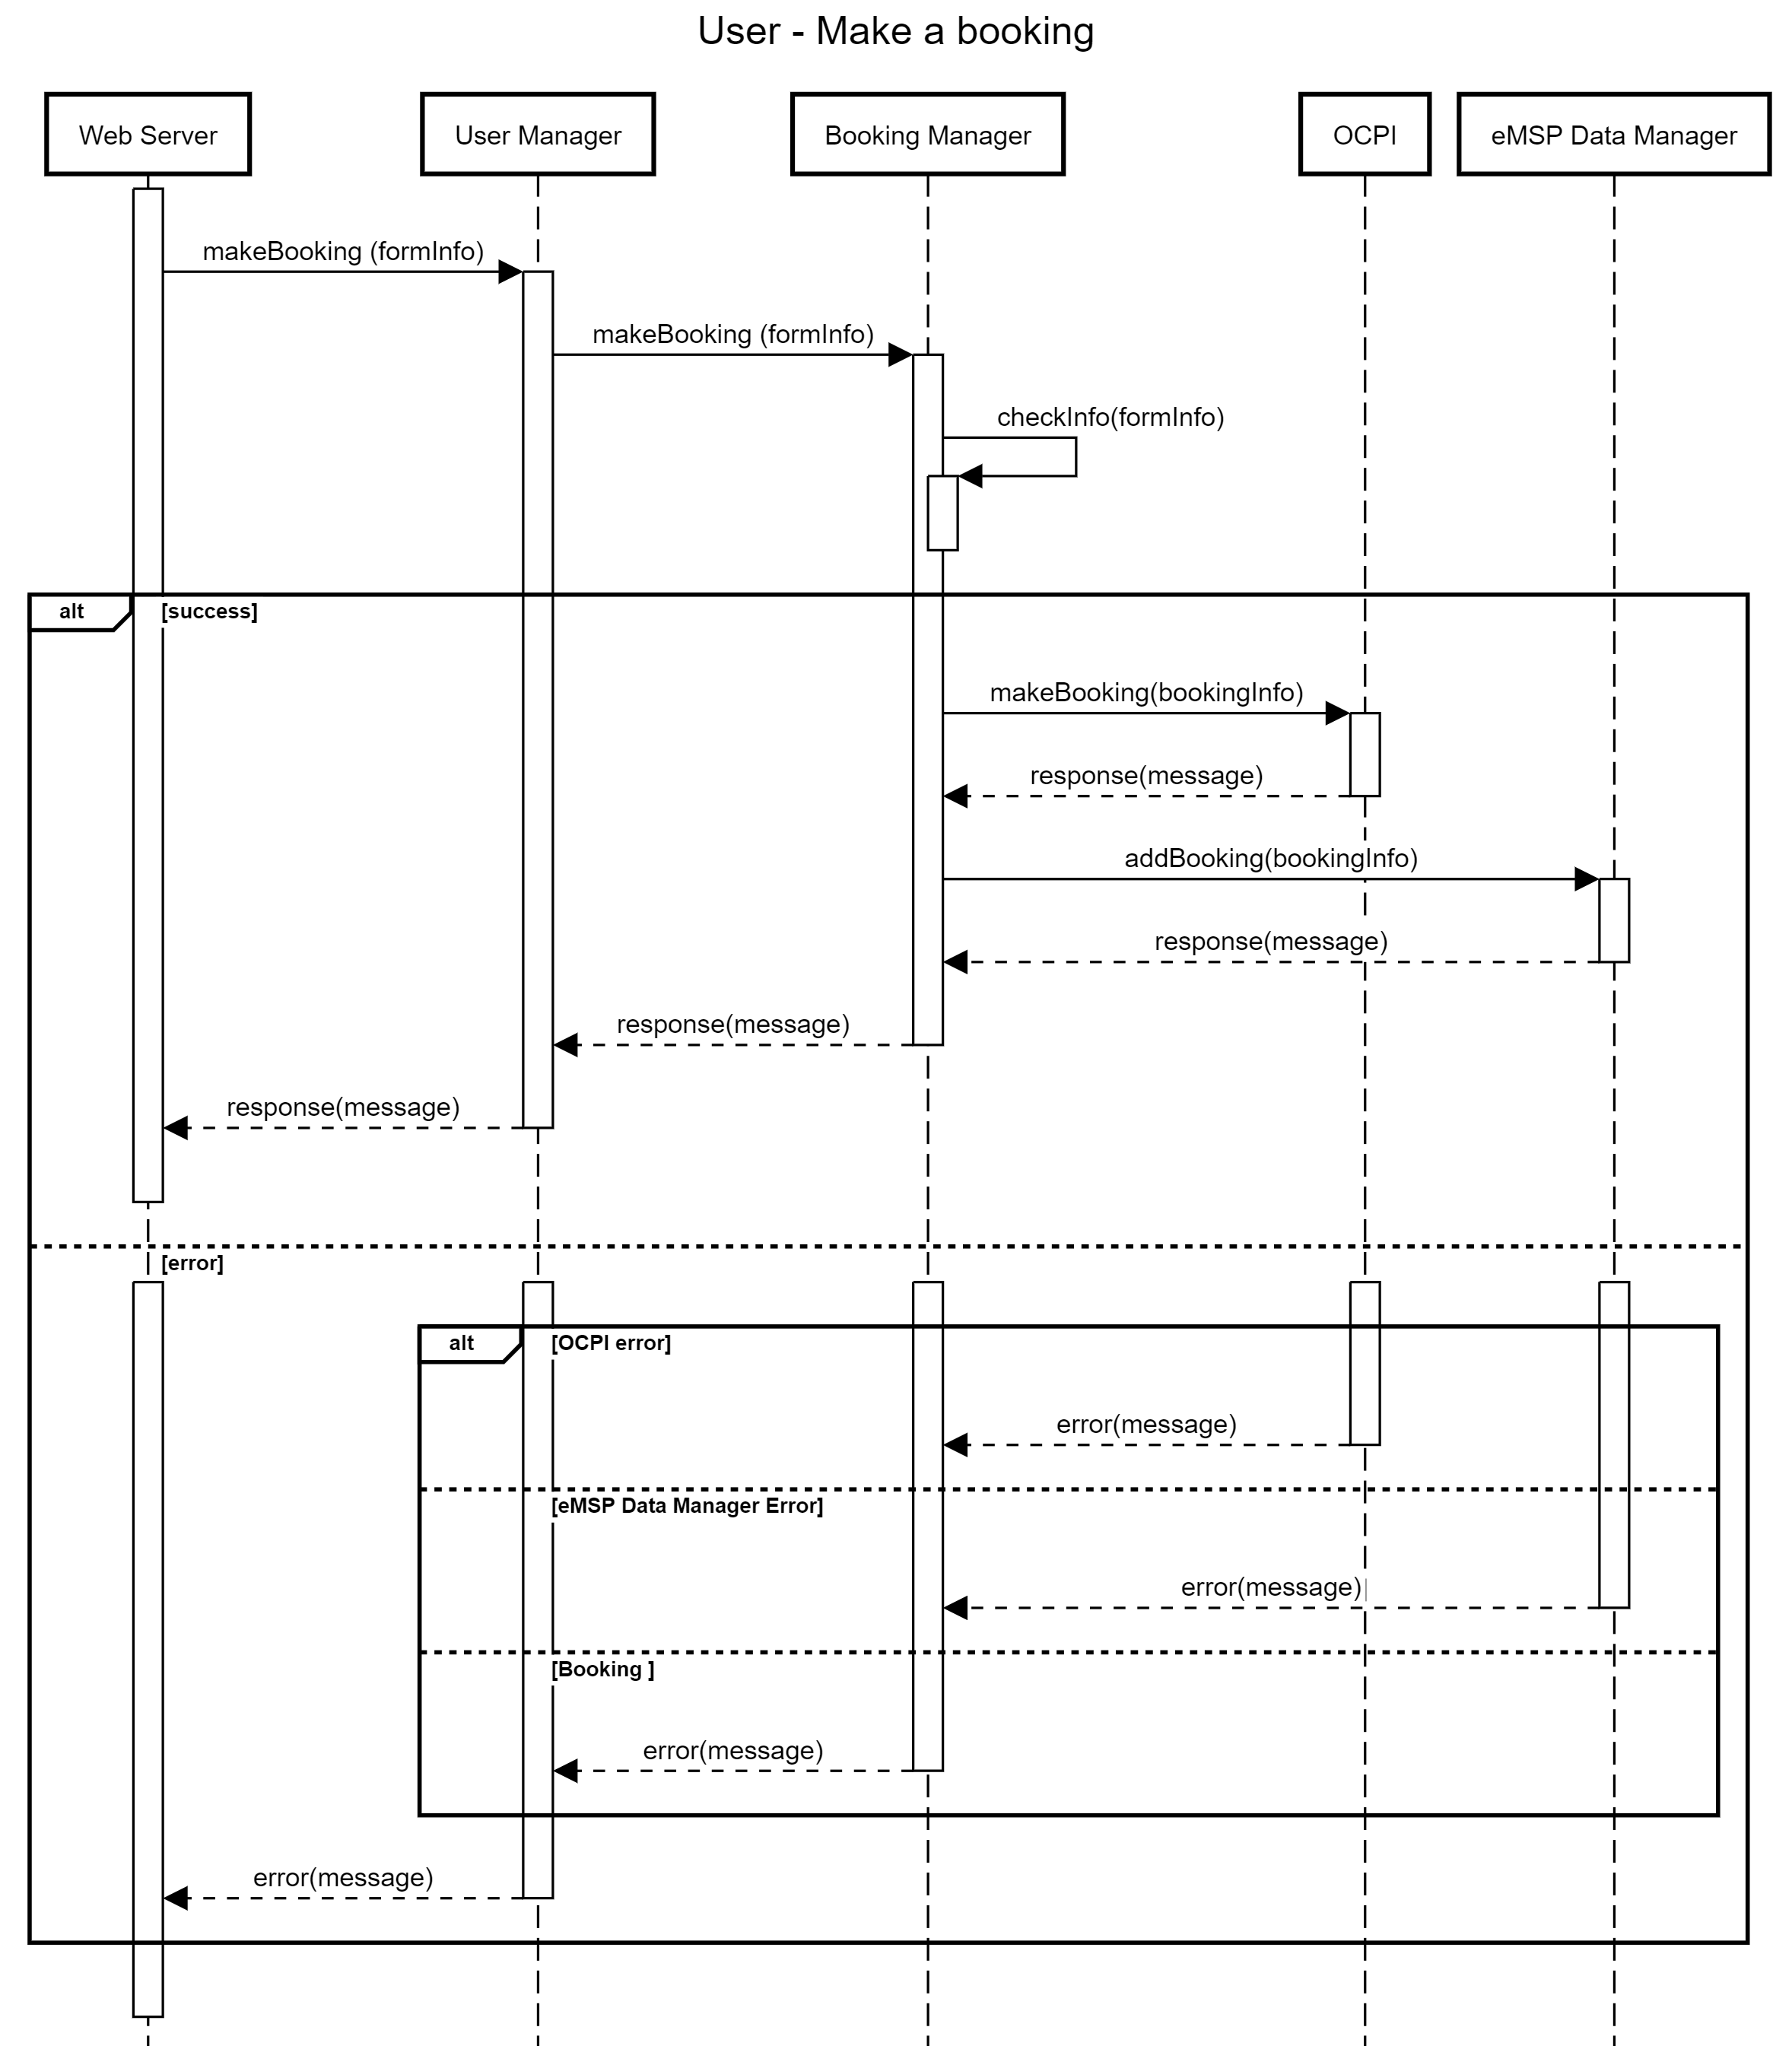
\includegraphics[scale=0.15, center]{assets/sequenceDiagrams/User Make Booking.png}
        \caption{Sign Up}
        \label{Make Booking}
    \end{figure}
\end{center}
This sequence displays how a user is able to insert a new booking from a form. The form is firstly sent to the Booking Manager, where a check for the validity of all the information is done. If it is all valid, the info is extrapolated and the 
booking is communicated to the OCPI. The booking info is later saved on the database through the eMSP Data Manager. For the sake of readability, all errors are collapsed in the end and explained here.
The first possible error is caused by checkInfo(), if the data inserted by the user is invalid. Lastly, an error could be raised by the OCPI if the booking doesn't go through for any reason. We assume the addition of the booking to the database doesn't cause errors.
\newline

\textbf{Book a map}\newline
We decided not to show book from map as it is basically the same as Make a Booking: it is still a form that has some fields precompiled when the button is pressed on the map.
\newpage

\textbf{Charging process}
\begin{center}
    \begin{figure}[H]
        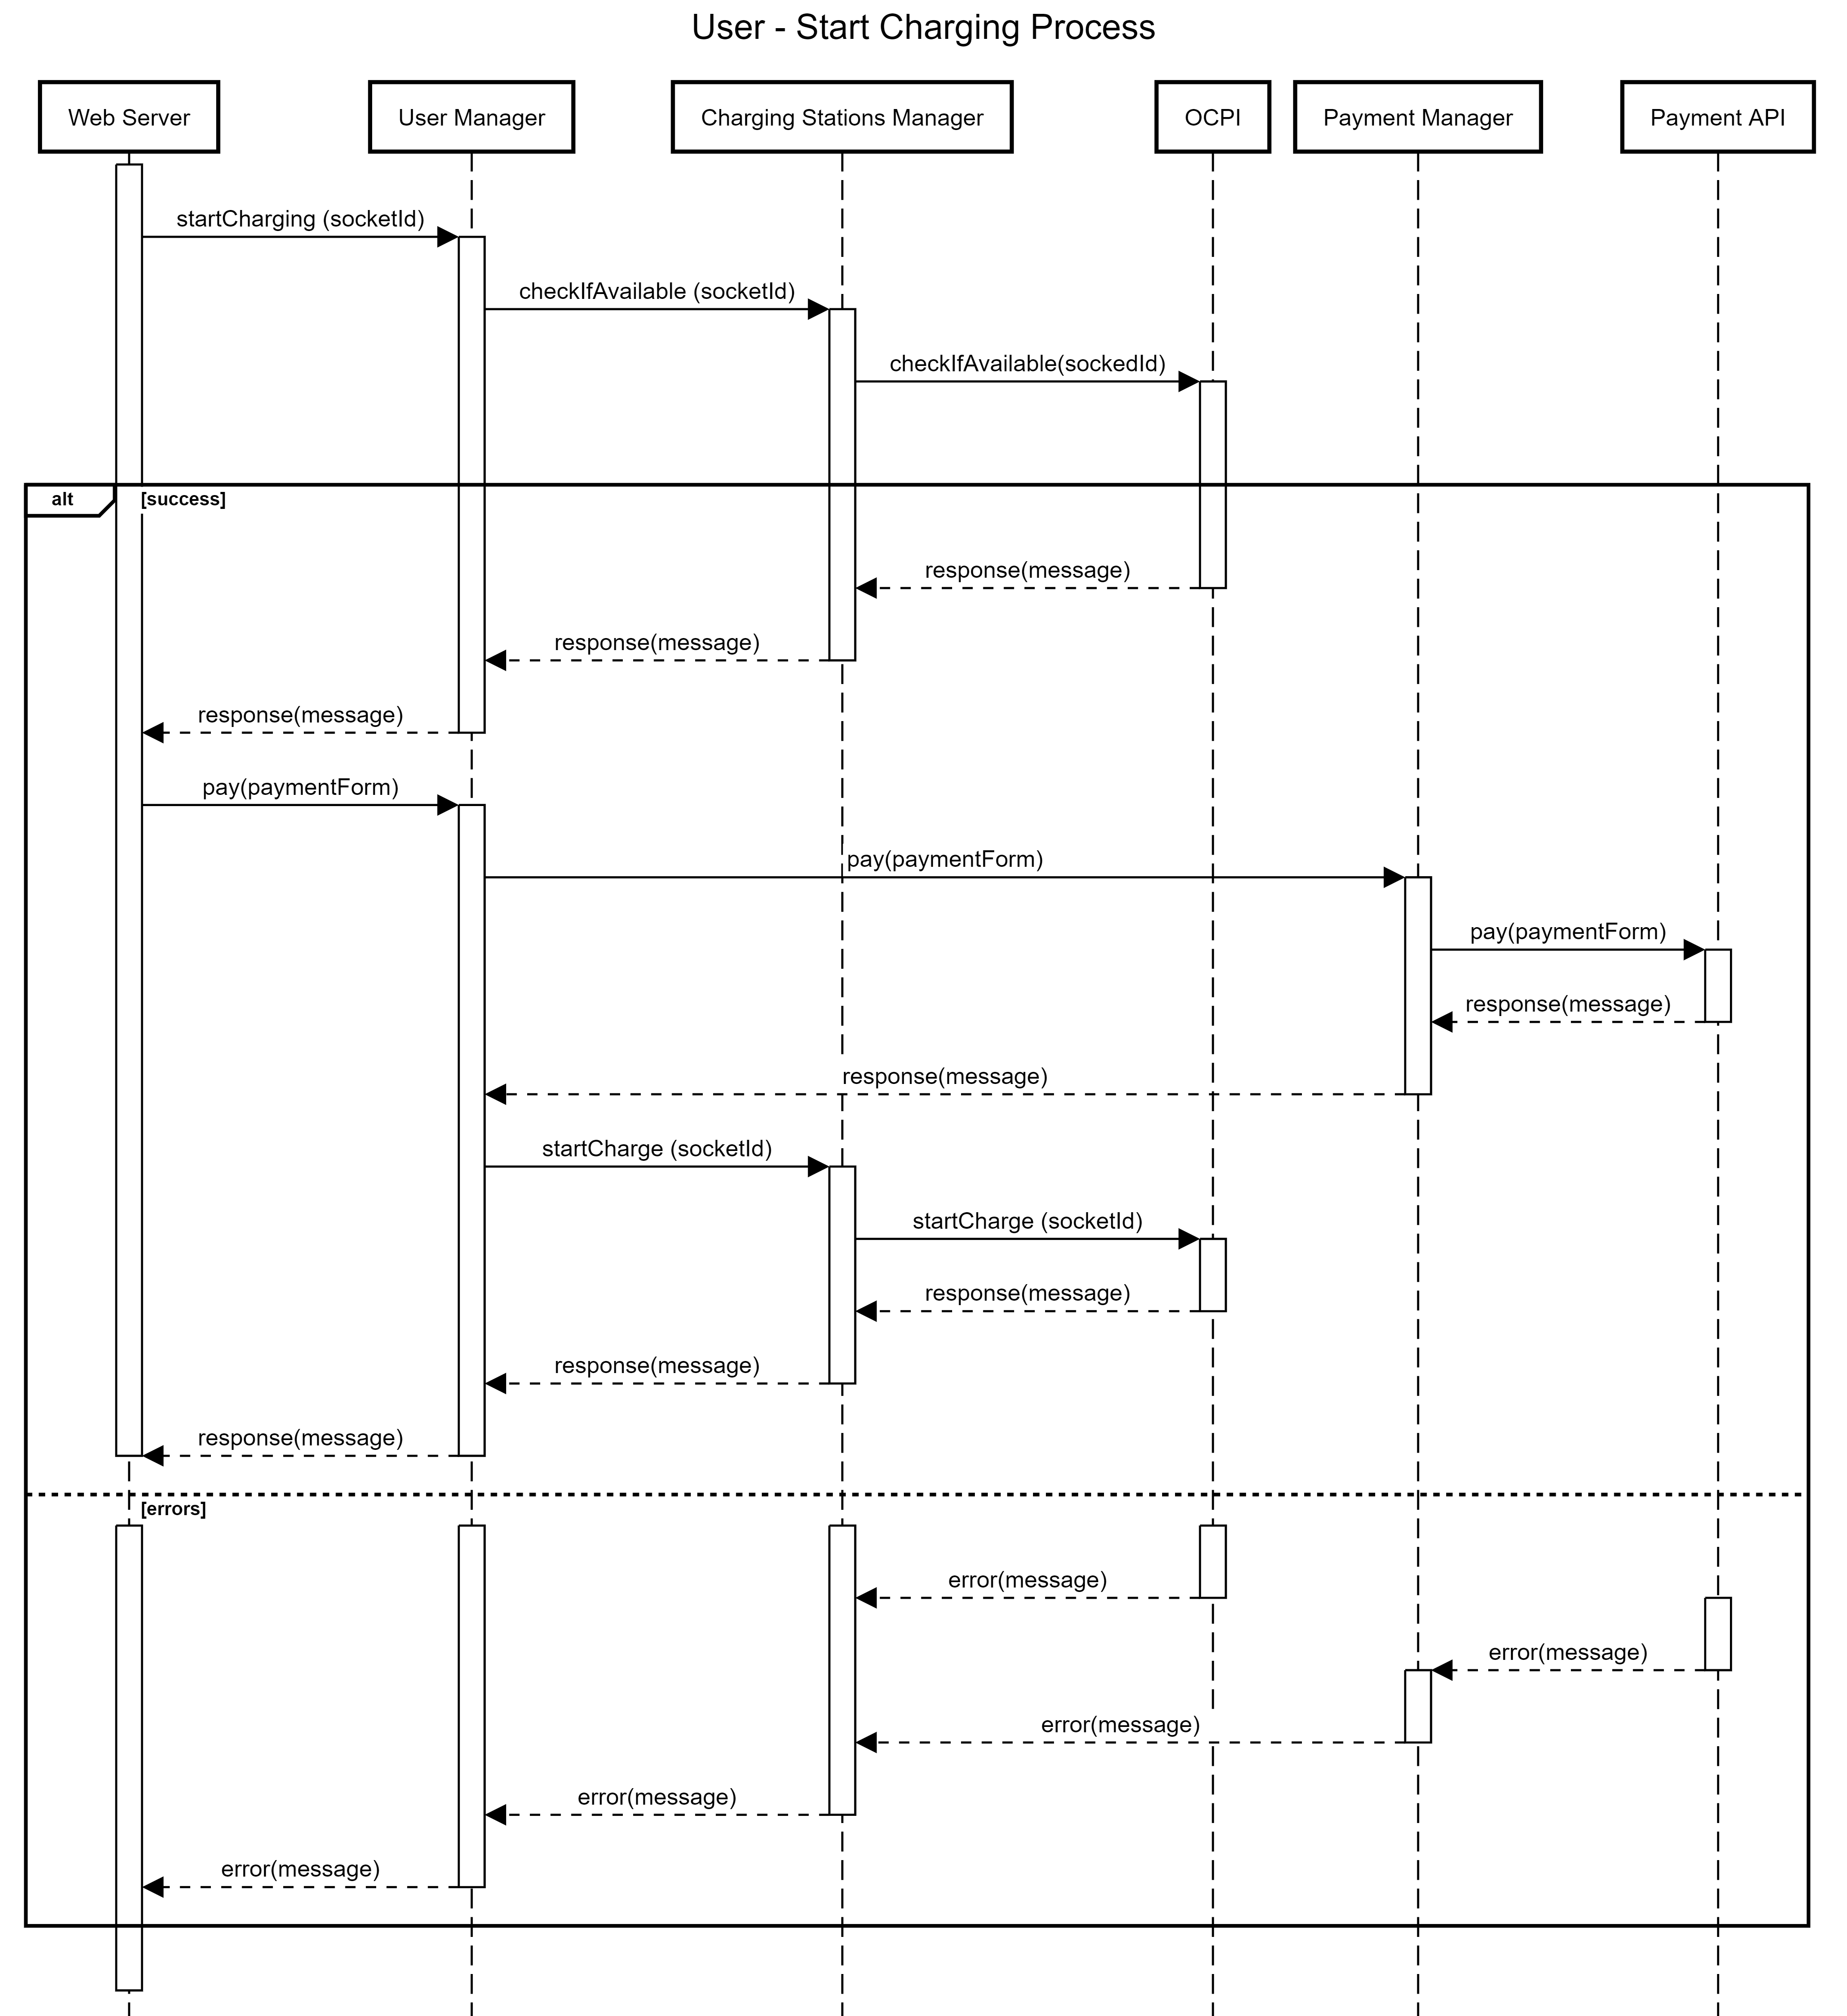
\includegraphics[scale=0.10, center]{assets/sequenceDiagrams/User Start Charging Process.png}
        \caption{Schedule suggestions}
        \label{Start Charging Process}
    \end{figure}
\end{center}
This sequence explains what happens after a User plugs his EV to a charging point and presses "Start charging" on the button of the respective socket. For the sake of readability, throughout the first part of the alt it is assumed all interactions end with success. Errors will be explained later.\newline
Firstly a socketID is sent to the Charging Stations Manager, to check whether the requested socket is available as it could be booked or unavailable. If the request is positive, the user is shown
a form for the payment that will be compiled and sent back to the Payment Manager. The Payment Manager will proceed to send the information to the Payment API that will actuate the actual payment.
When the payment goes through, the User Manager will communicate to the OCPI through the Charging Stations Manager that the charge can start. The OCPI will then send data regarding the status back to the User.
The errors will be now explained more thorougly. Firstly, an error could be raised by the OCPI in case the requested socket is not currently available.
Secondly, an error could be caused by the Payment Manager in the case the payment Form contains invalid data. The third error could be raised by the Payment API in case the payment process doesn't end successfully.
It is important to note that we assume that once the user has payed the OCPI cannot fail in starting the charge, as its availability was checked beforehand. If this wasn't the case, there could be instances where the User pays and the charge doesn't actually start.

\newpage
\textbf{Schedule suggestions}
\begin{center}
    \begin{figure}[H]
        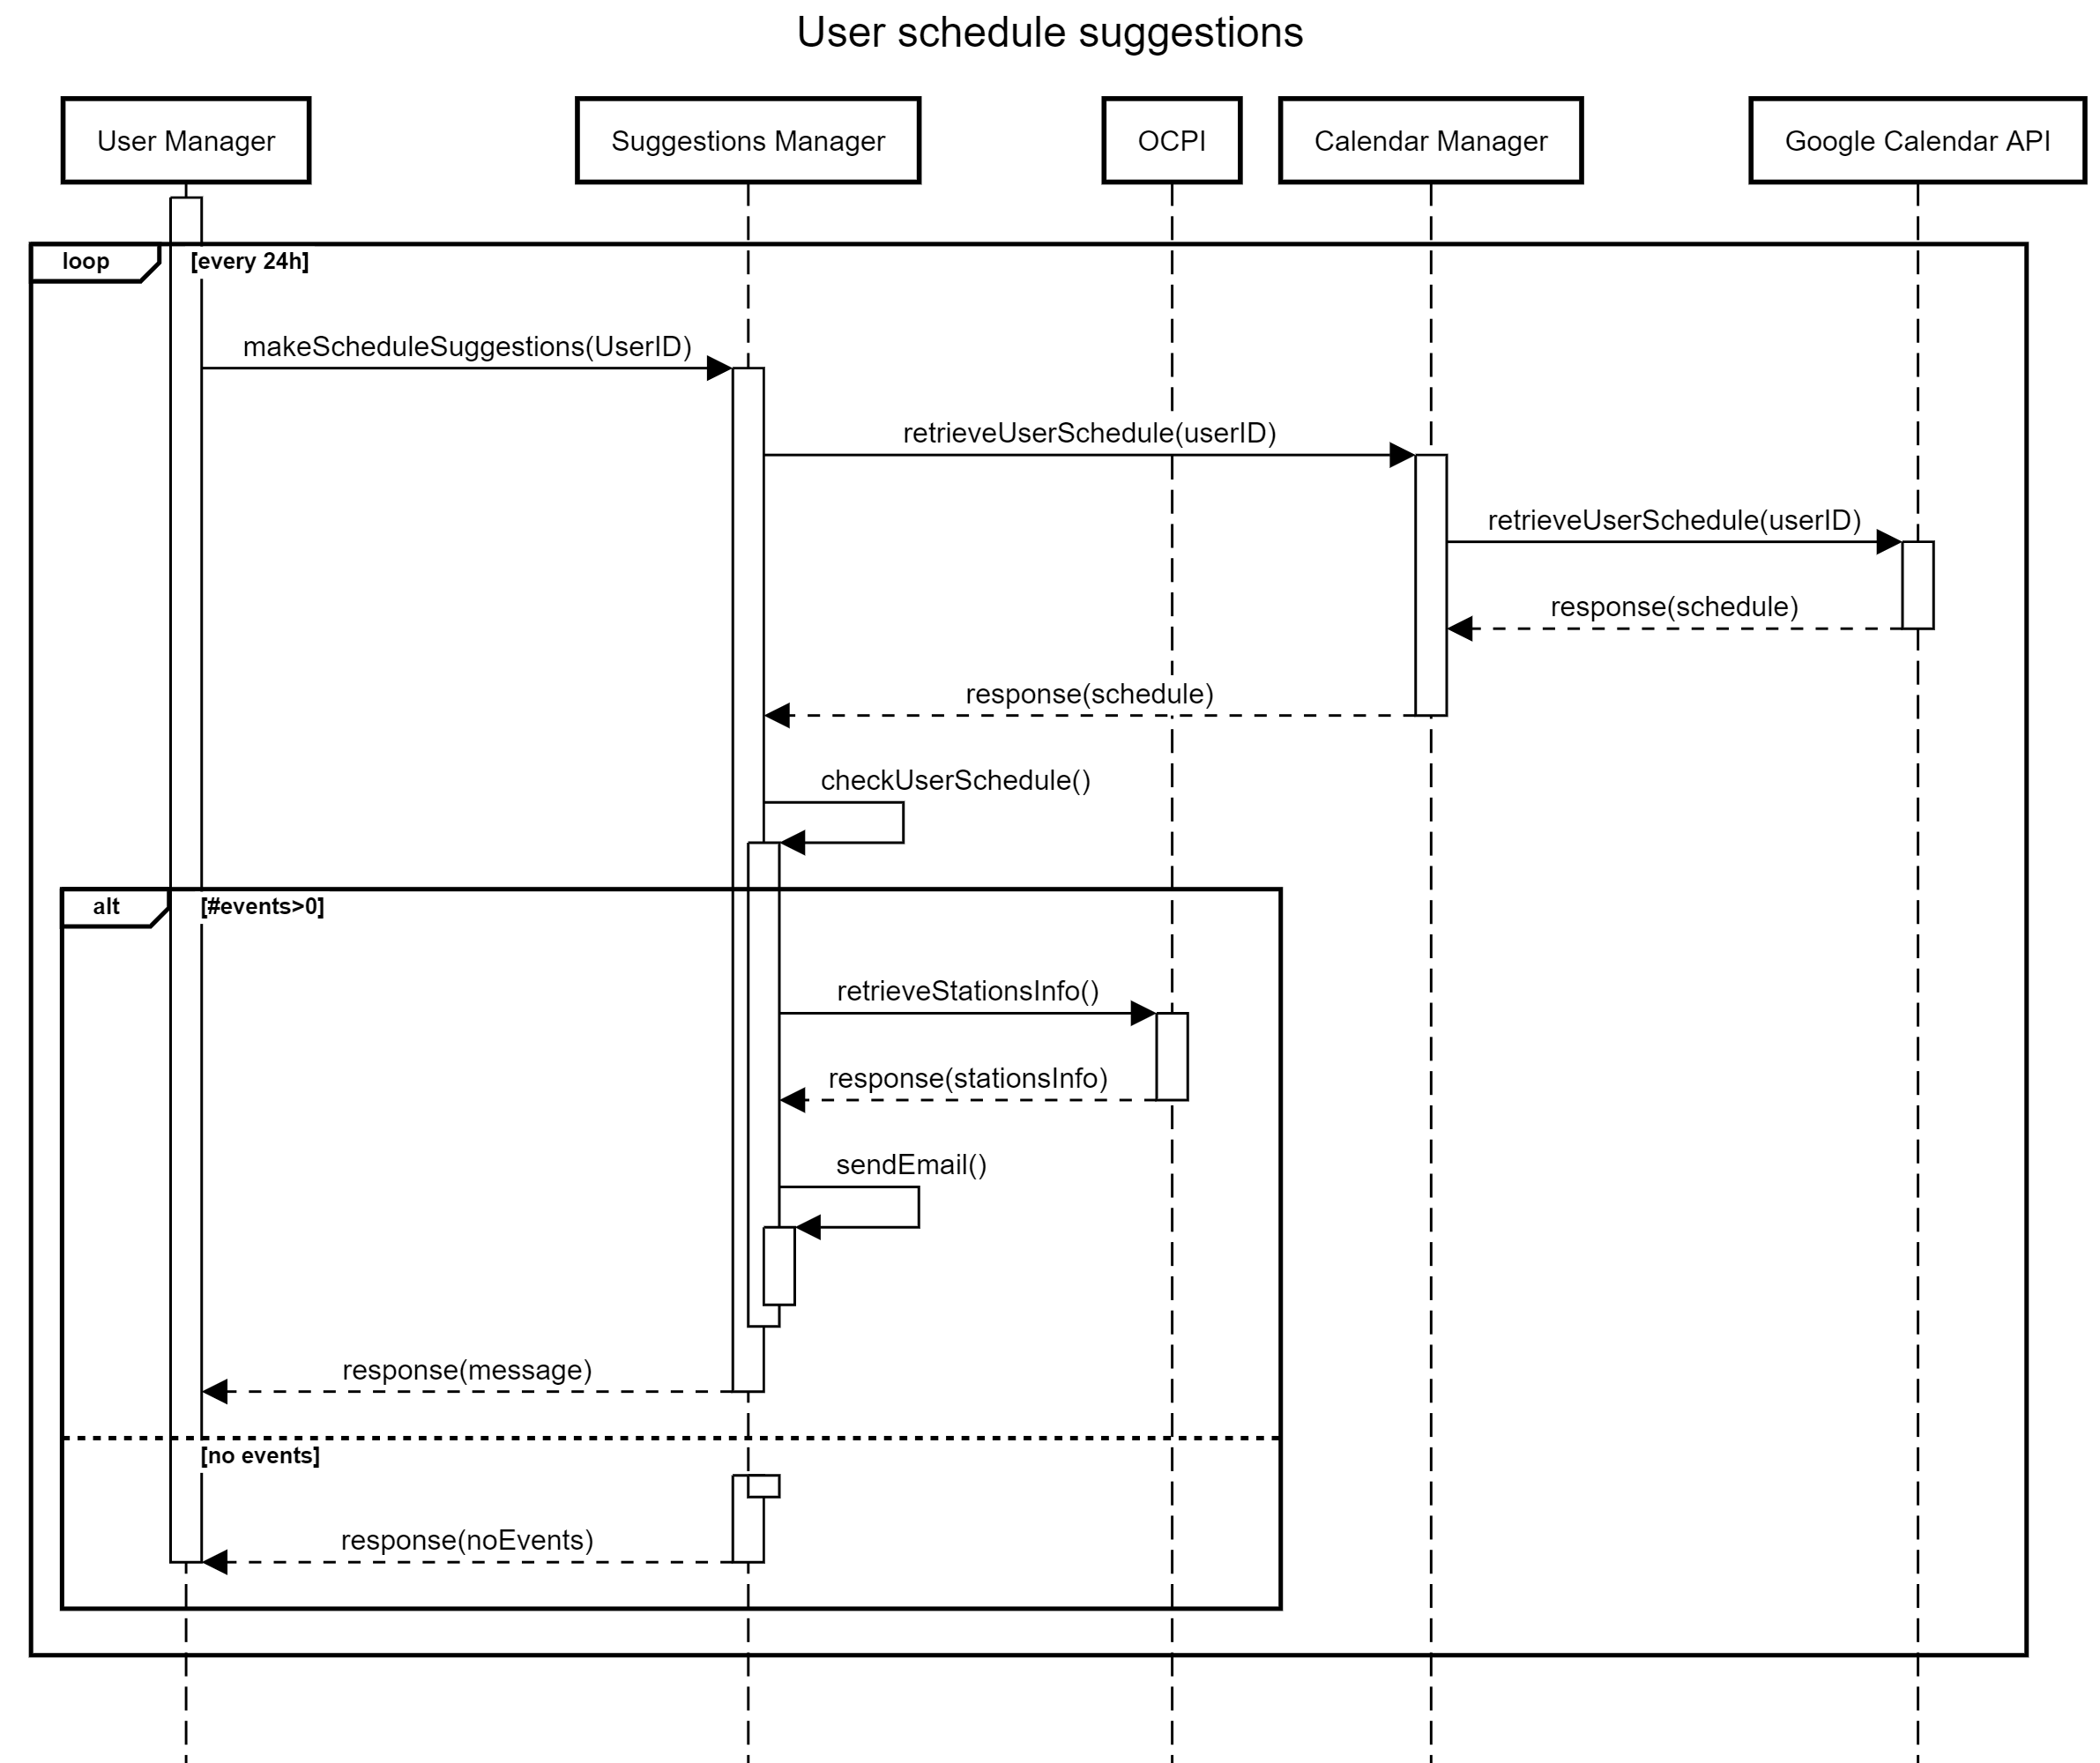
\includegraphics[scale=0.20, center]{assets/sequenceDiagrams/User schedule suggestions.png}
        \caption{Schedule suggestions}
        \label{Schedule suggestions}
    \end{figure}
\end{center}
\newpage
The user's schedule suggestion service triggers a check every day at 00:00 to see if the user has planned some events for the next day.
When it triggers, the SuggestionManager calls the CalendarManager in order to retrieve the user's schedule for the next day by using the Google Calendar API.
Then the SuggestionManager checks all the new events: if there is at least one event it retrieves a list of charging stations information that are nearby the event's location by communicating with the OCPI component, and then sends an eMail with a list of charging stations based on their distance, cost and special offers.
The email will contain a link for each station that will redirect the user to a pre-filled booking form, in order to easily book a socket.
\newpage

\textbf{Battery suggestion}
\begin{center}
    \begin{figure}[H]
        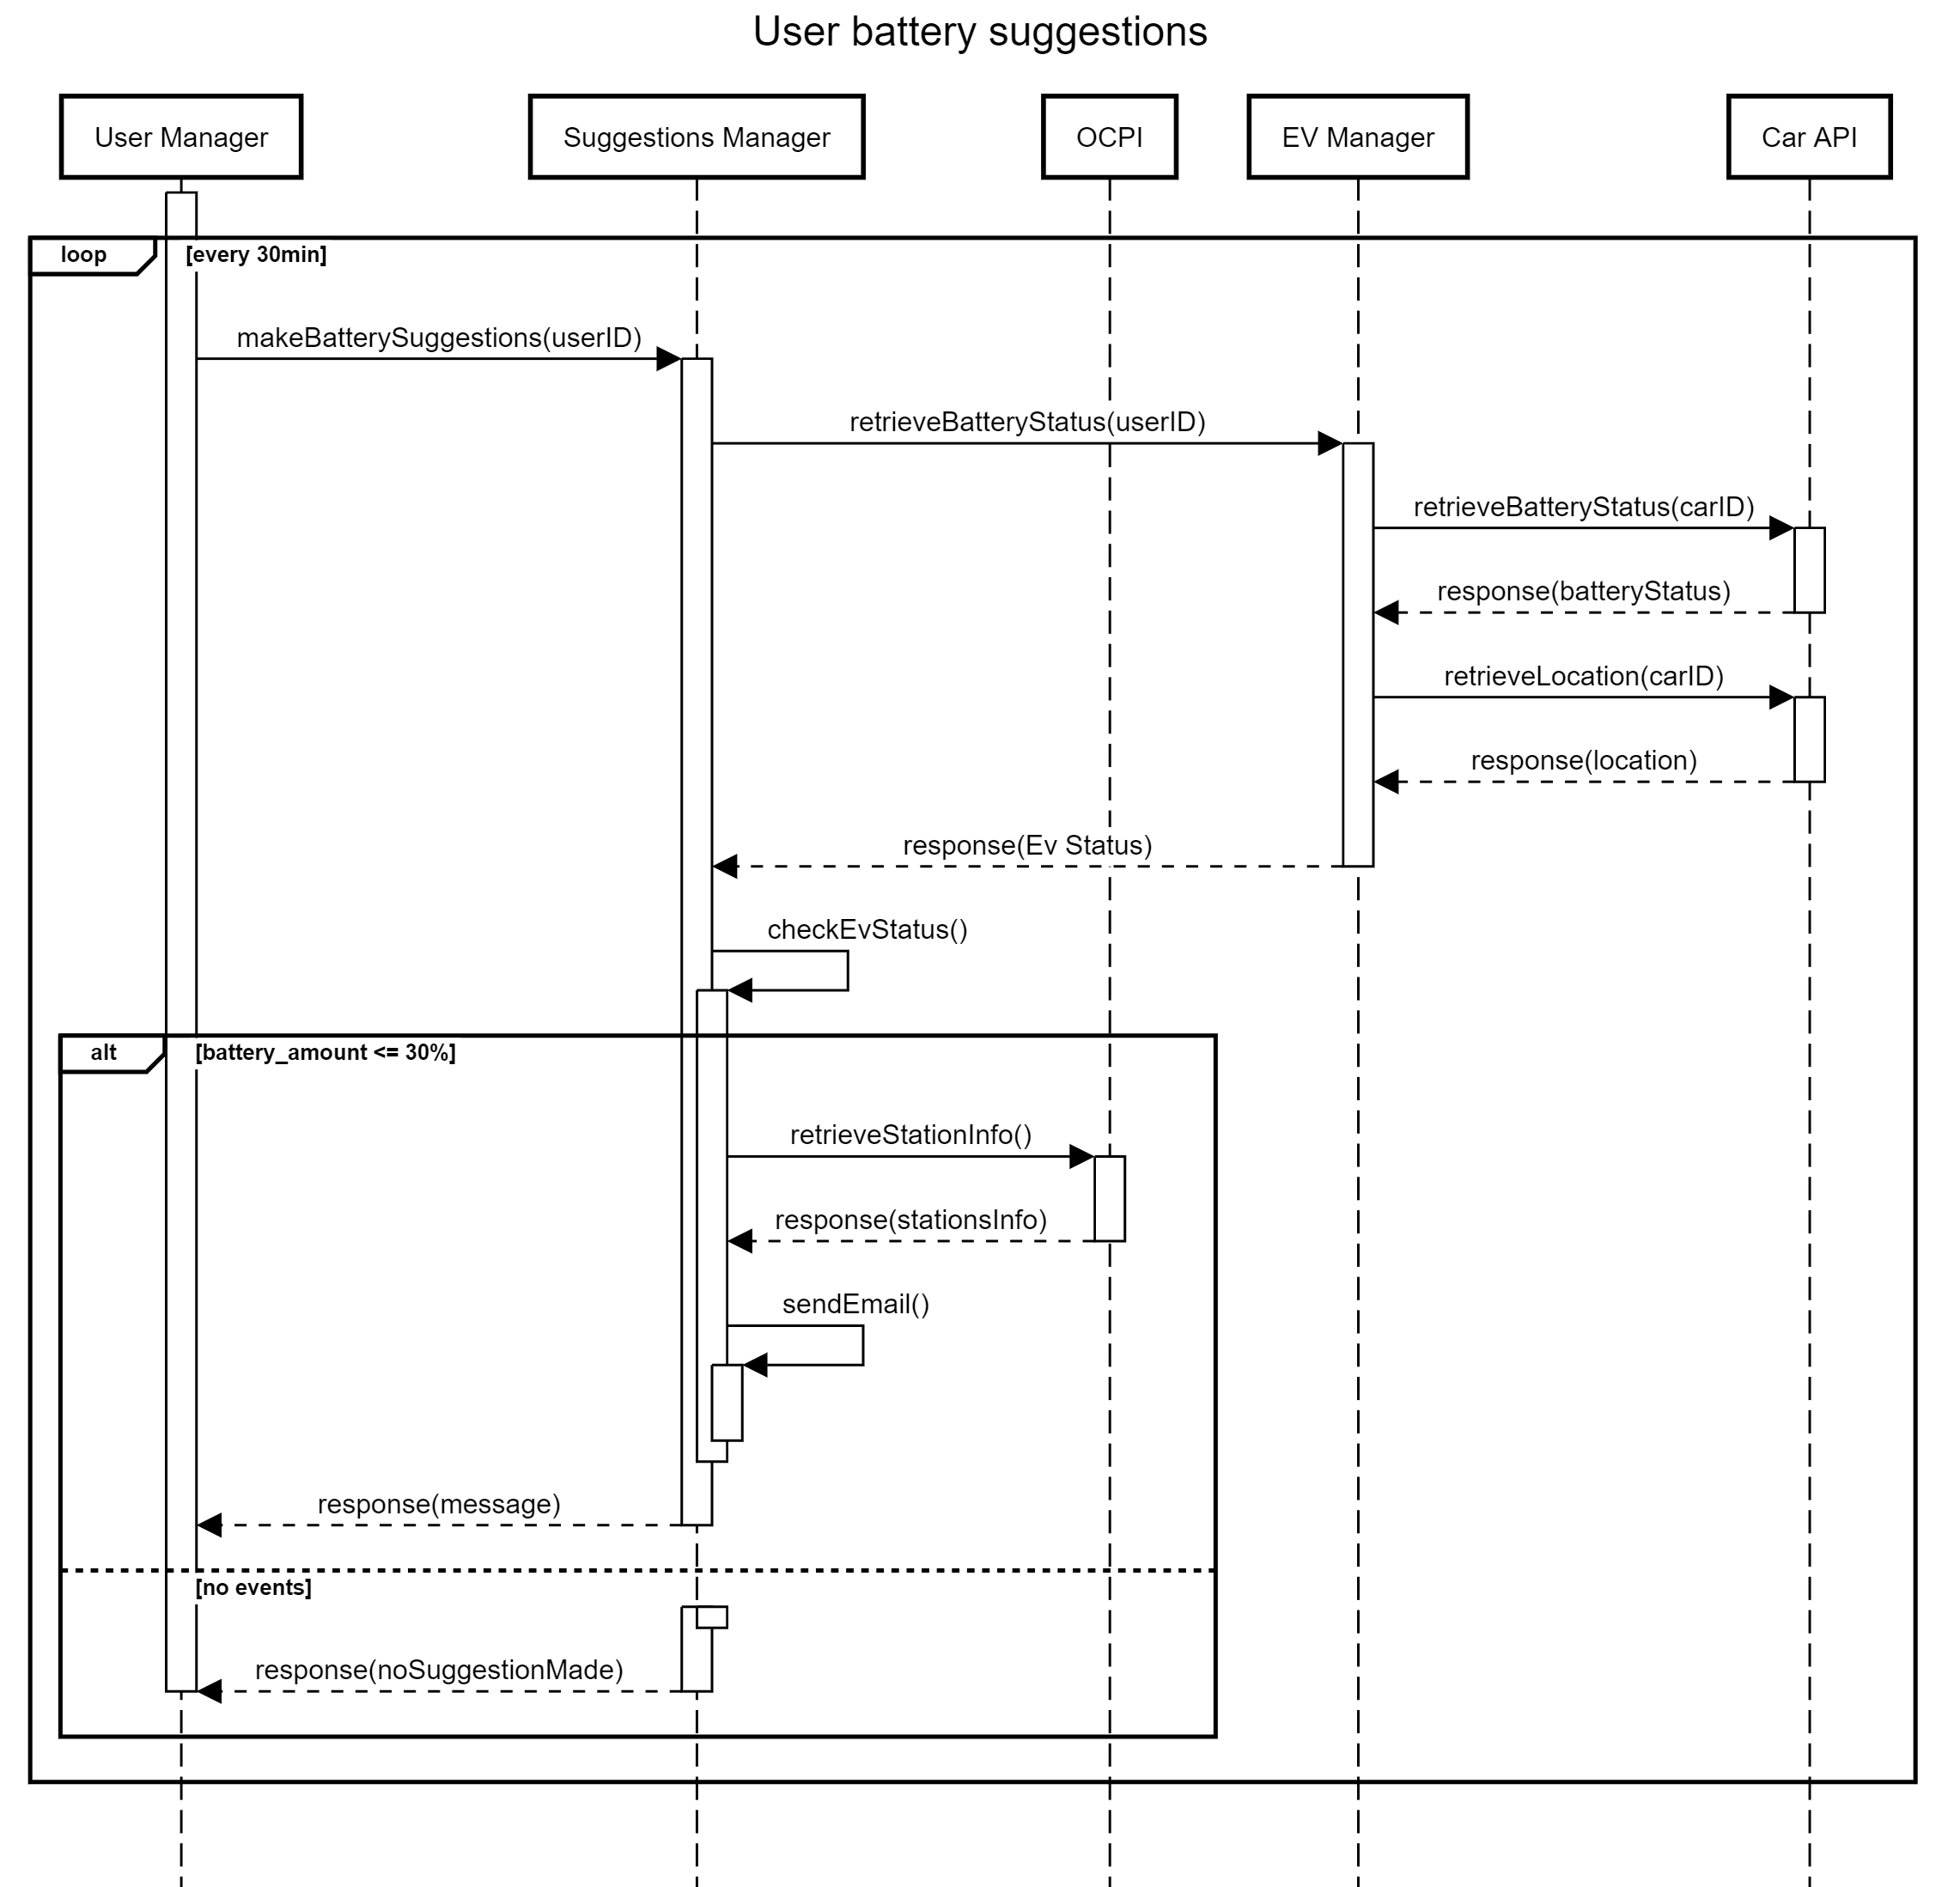
\includegraphics[scale=0.20, center]{assets/sequenceDiagrams/battery suggestions.png}
        \caption{Battery suggestion}
        \label{Battery suggestion}
    \end{figure}
\end{center}
\newpage
The battery suggestion service triggers a check every 30 minutes to see if the user'EV has battery status below a certain threshold.
When it triggers, the SuggestionManager calls the EVManager in order to retrieve the user's car battery status and location by using the CarAPI.
Then the SuggestionManager checks the battery status: if it's below a certain threshold it retrieves a list of charging stations information that are nearby the user's home or the car location by communicating with the OCPI component, and then sends an eMail with a list of charging stations based on their distance, cost and special offers.
Note that this service is available only for the users that have a car registered in the system and that have a brand that supports this features with their API.
\newpage

\underline{\textbf{CPOW diagrams}}\\
\textbf{Insert discount}
\begin{center}
    \begin{figure}[H]
        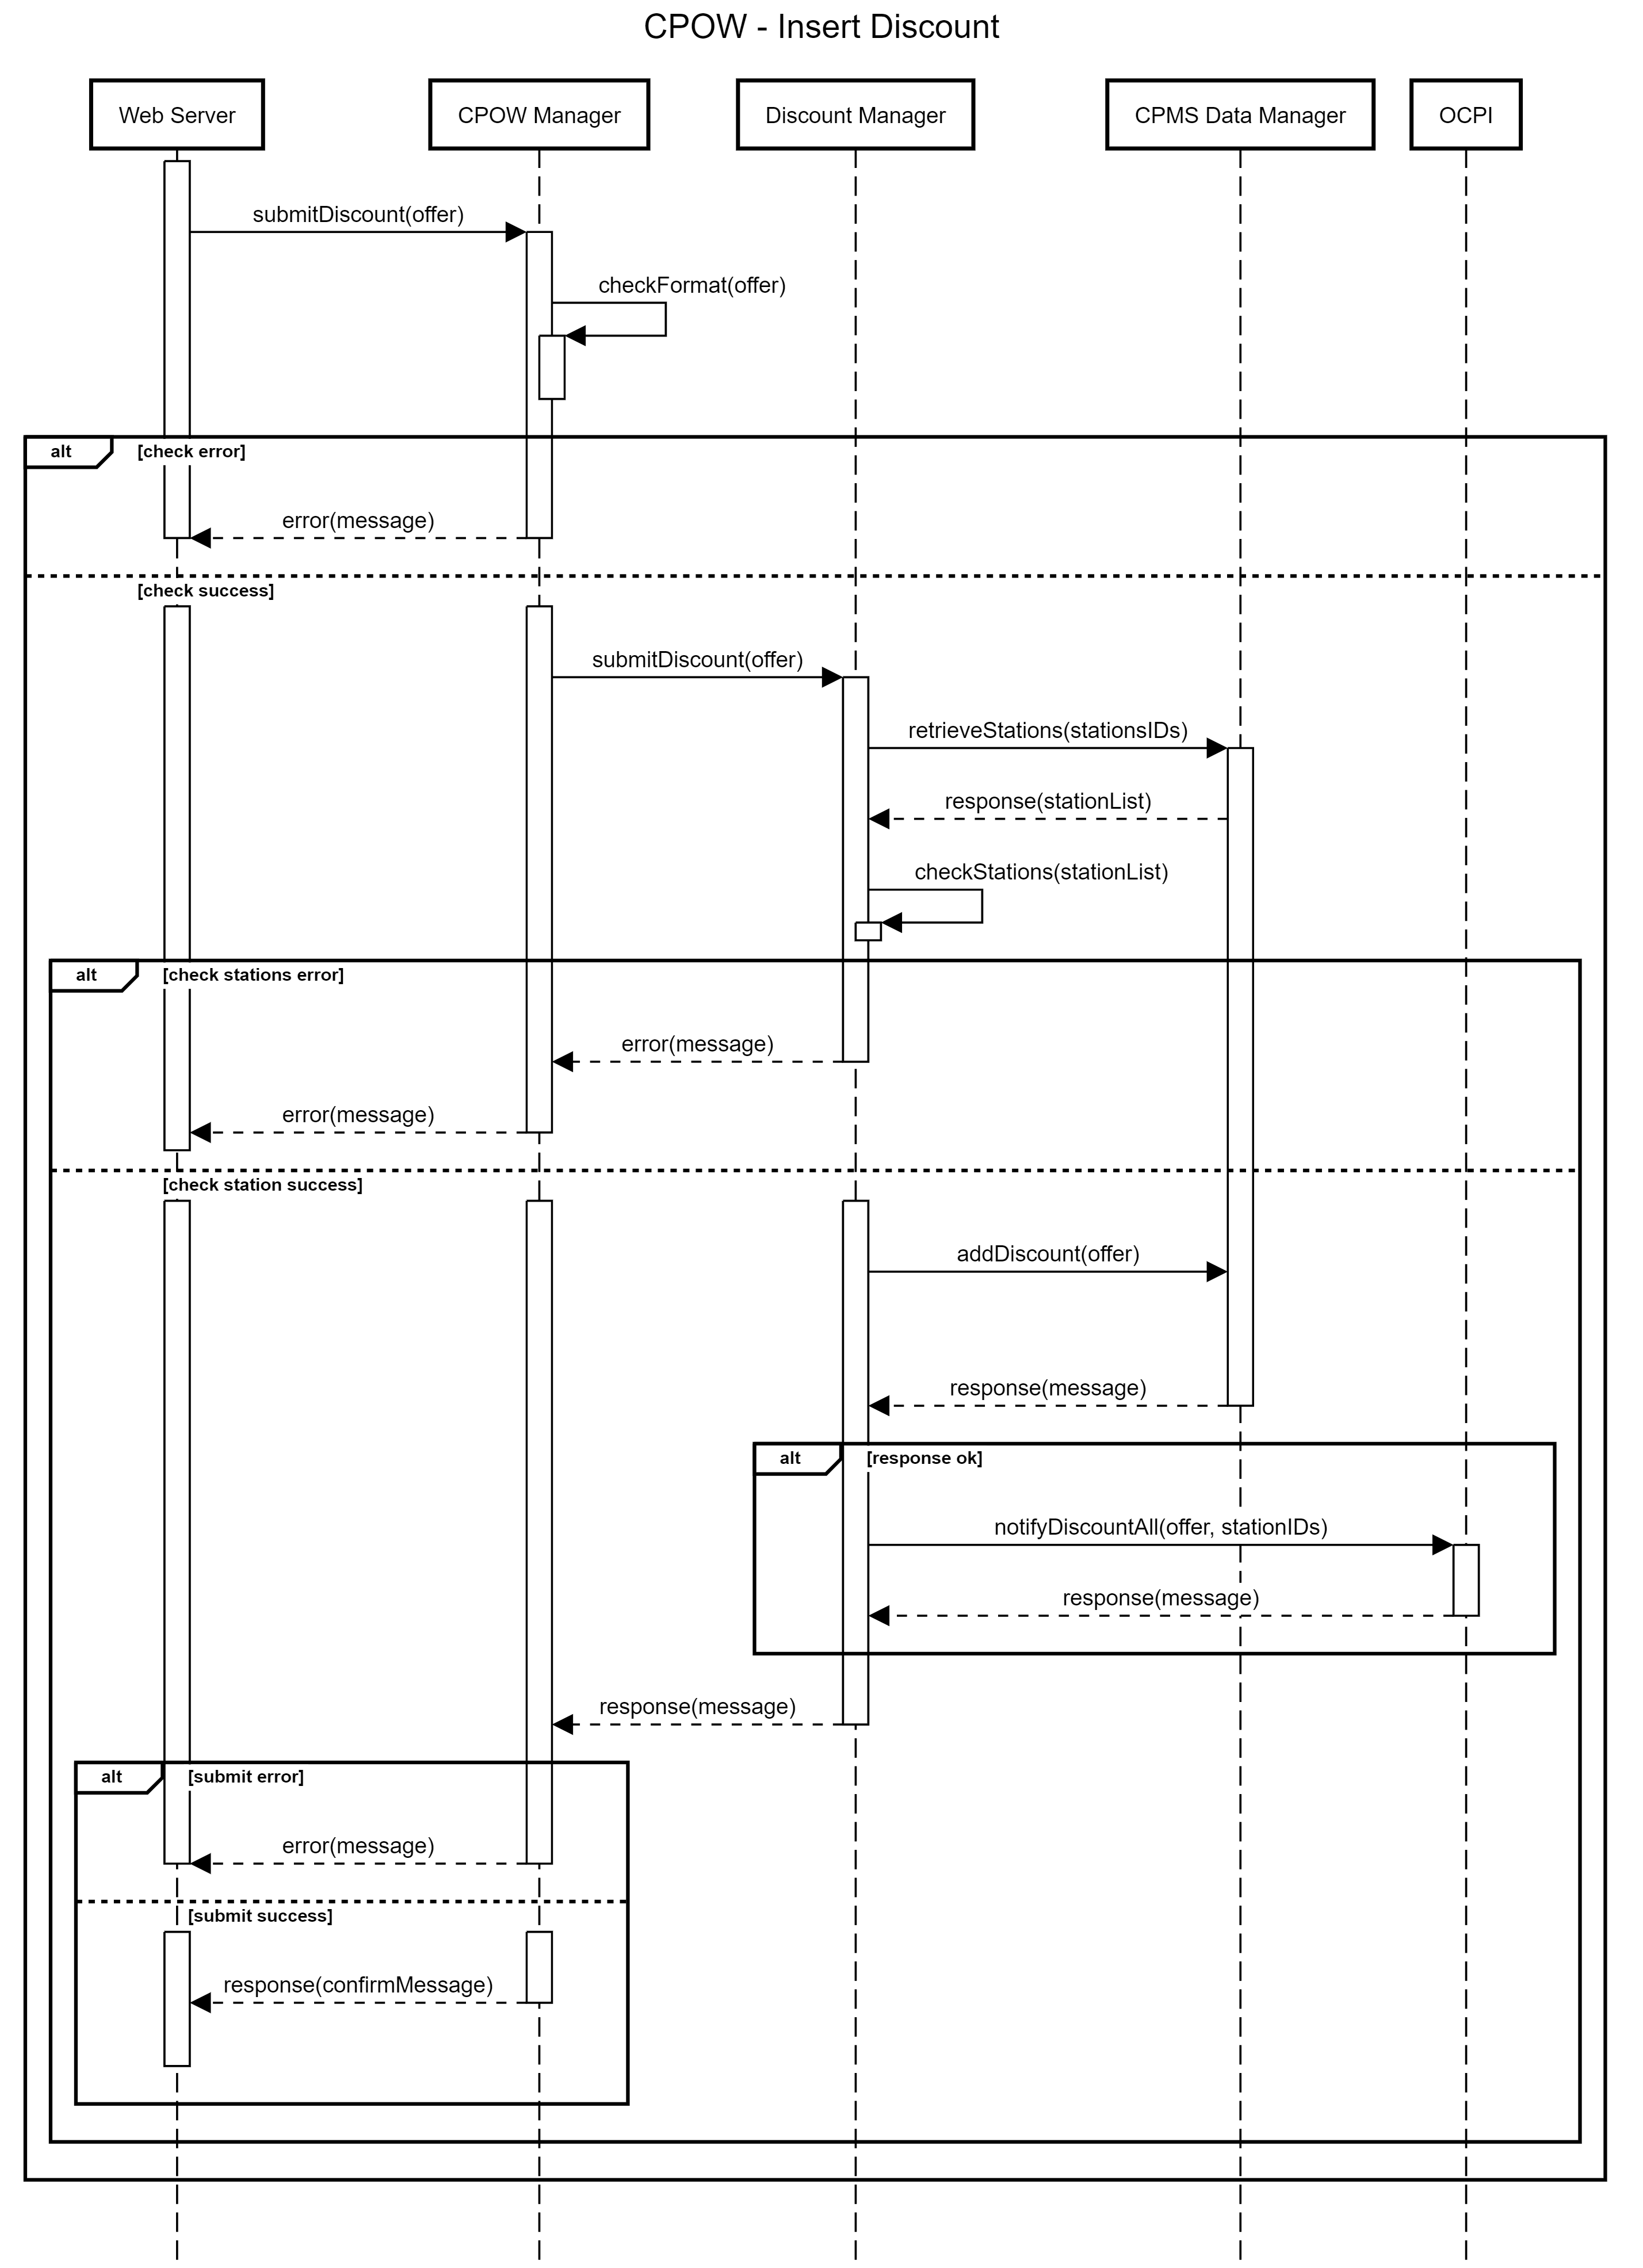
\includegraphics[scale=0.12, center]{assets/sequenceDiagrams/CPOW insert discount.png}
        \caption{CPOW - Insert discount}
        \label{CPOW - Insert discount}
    \end{figure}
\end{center}
The insert discount interaction triggers when a CPOW wants to insert a new discount for a list of charging stations.
After receiving the form information, the CPOW Manager calls the Discount Manager in order to check if the stations are valid and if the discount is valid.
Then the discount is inserted in the database and the Discount Manager calls the OCPI component in order to notify all EMSPs that are connected to the CPMS about the new discount.
Note that in this diagram it is not showed the interaction with the OCPP component because it will apply the discount to the charging stations only when the discount's start date is reached.
\newpage

\textbf{Delete discount}
\begin{center}
    \begin{figure}[H]
        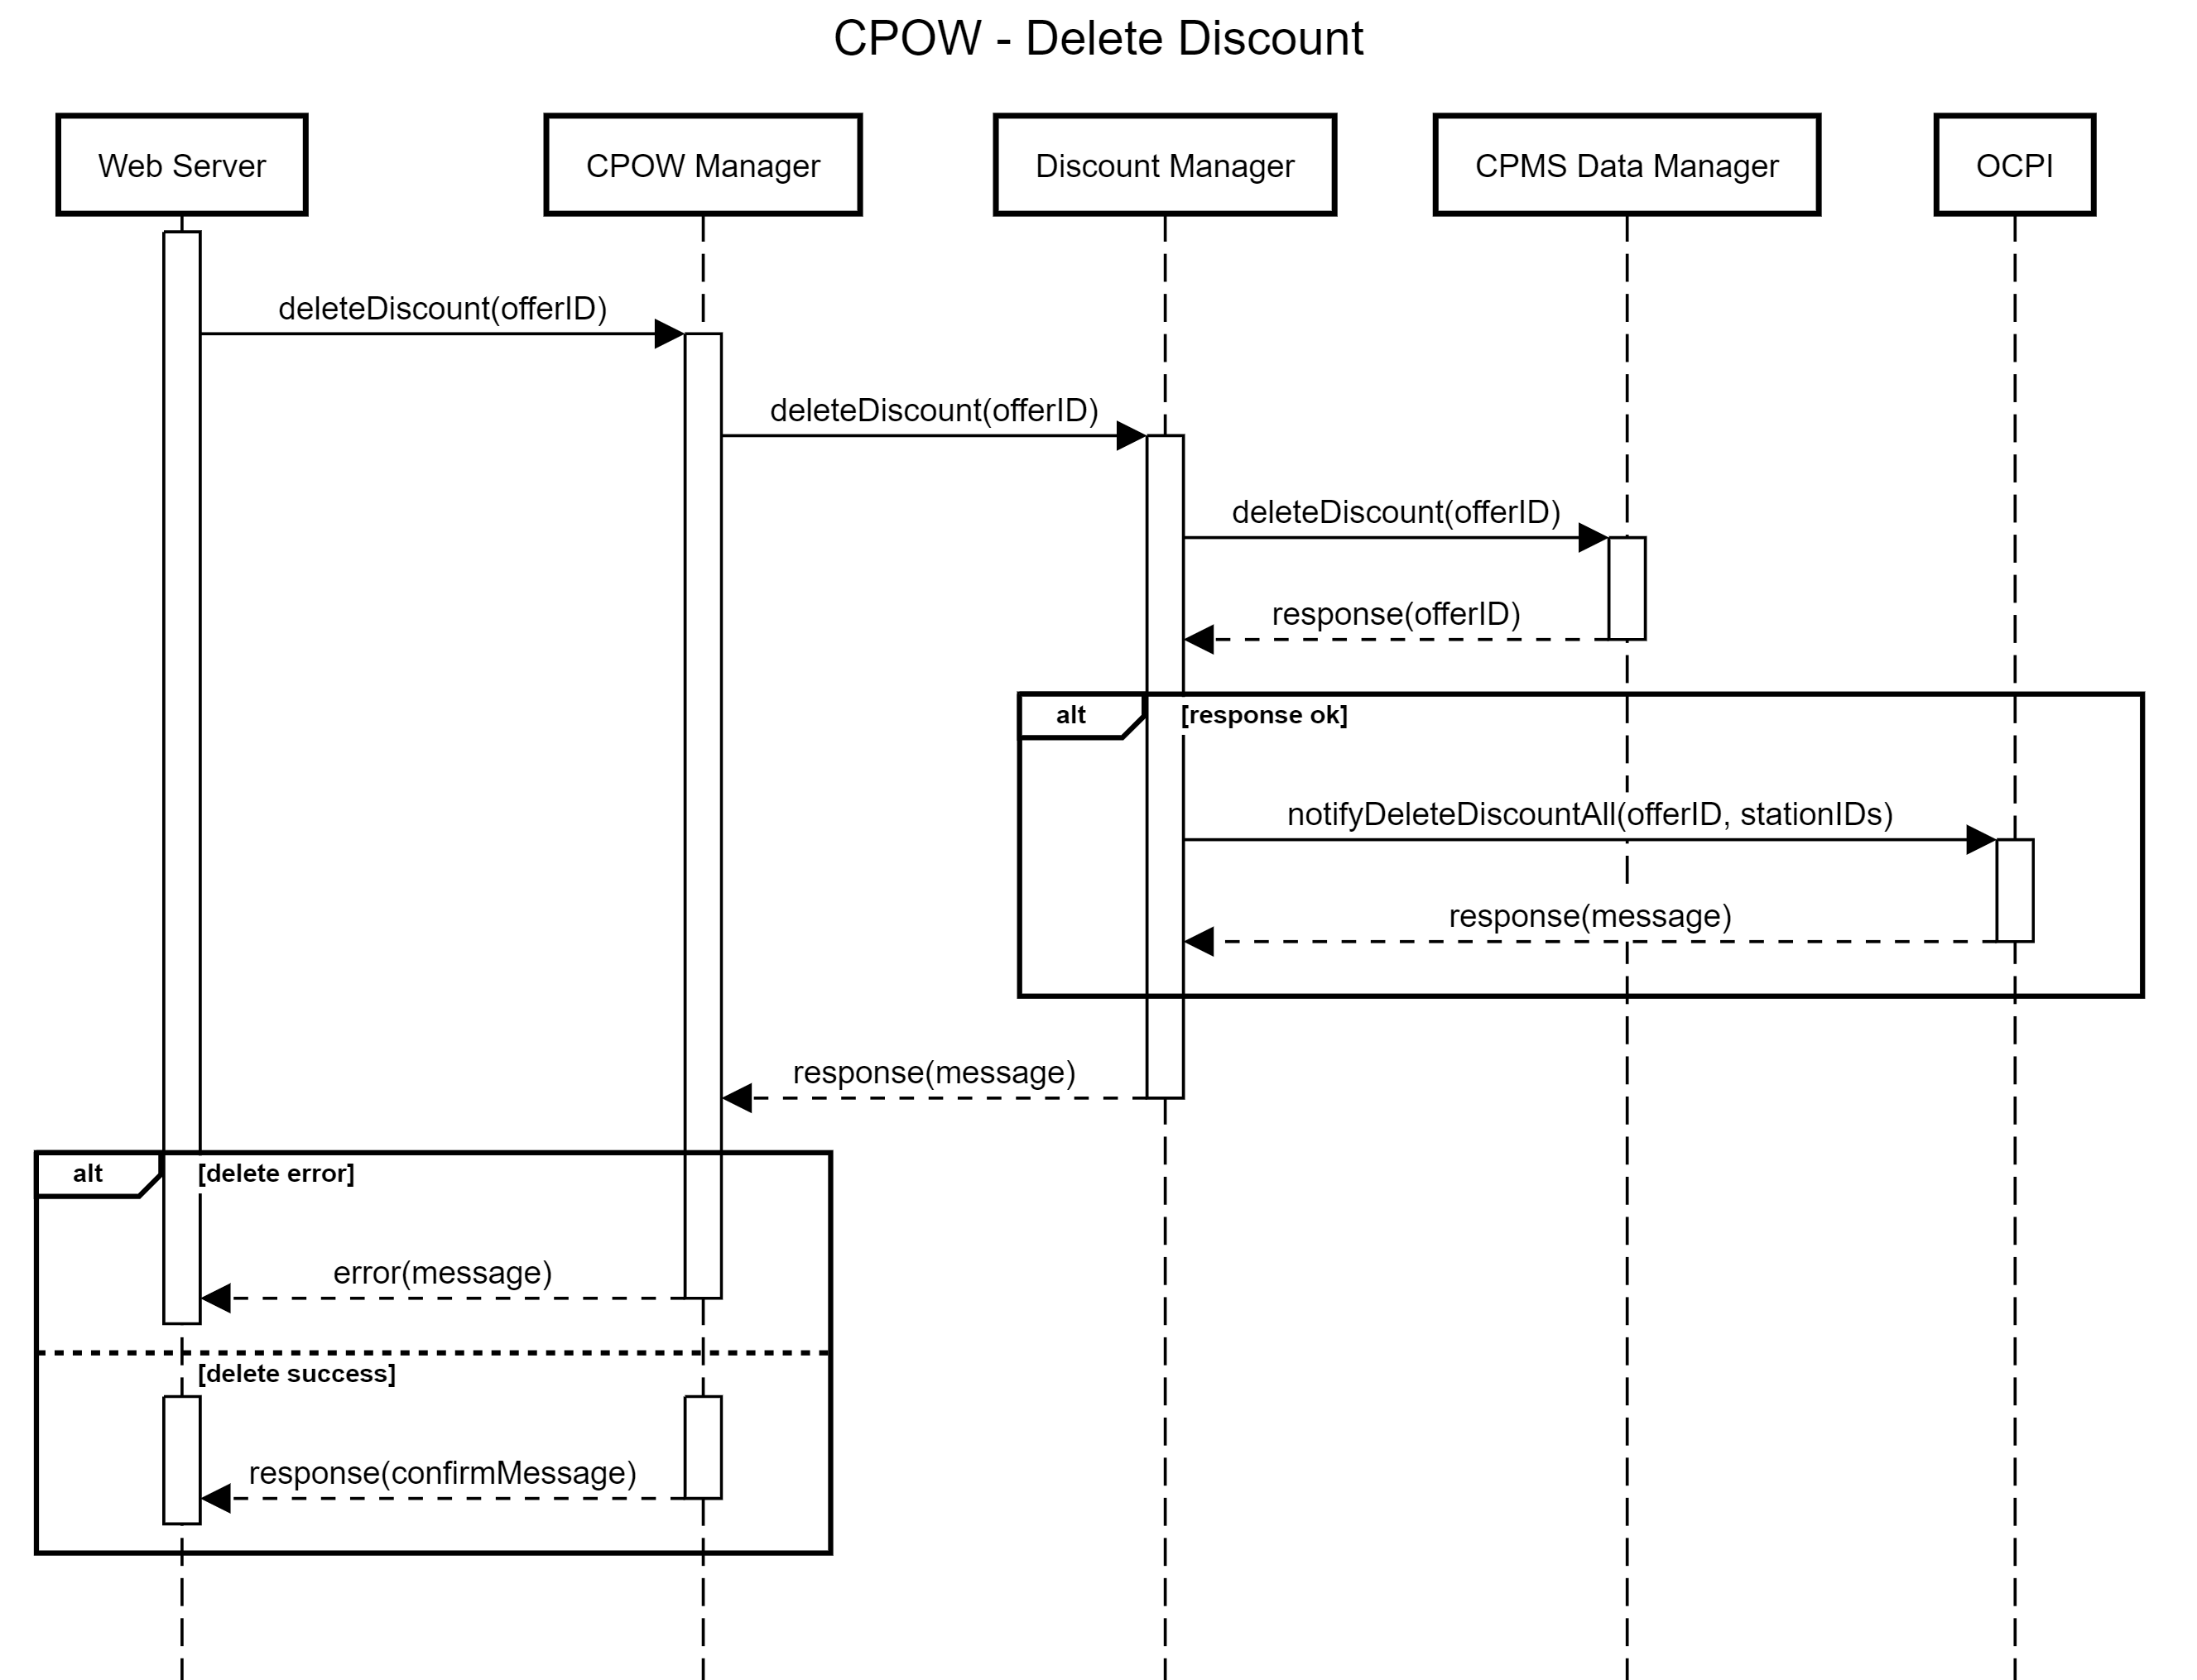
\includegraphics[scale=0.15, center]{assets/sequenceDiagrams/CPOW delete discount.png}
        \caption{CPOW - Delete discount}
        \label{CPOW - Delete discount}
    \end{figure}
\end{center}
The delete discount interaction triggers when a CPOW wants to delete a discount for all the charging stations to which it was applied.
After receiving the discountID, the system will check if the discount exists. If it is, it will delete it from the database and notify all EMSPs that are connected to the CPMS.
\newpage

\textbf{View charging stations}
\begin{center}
    \begin{figure}[H]
        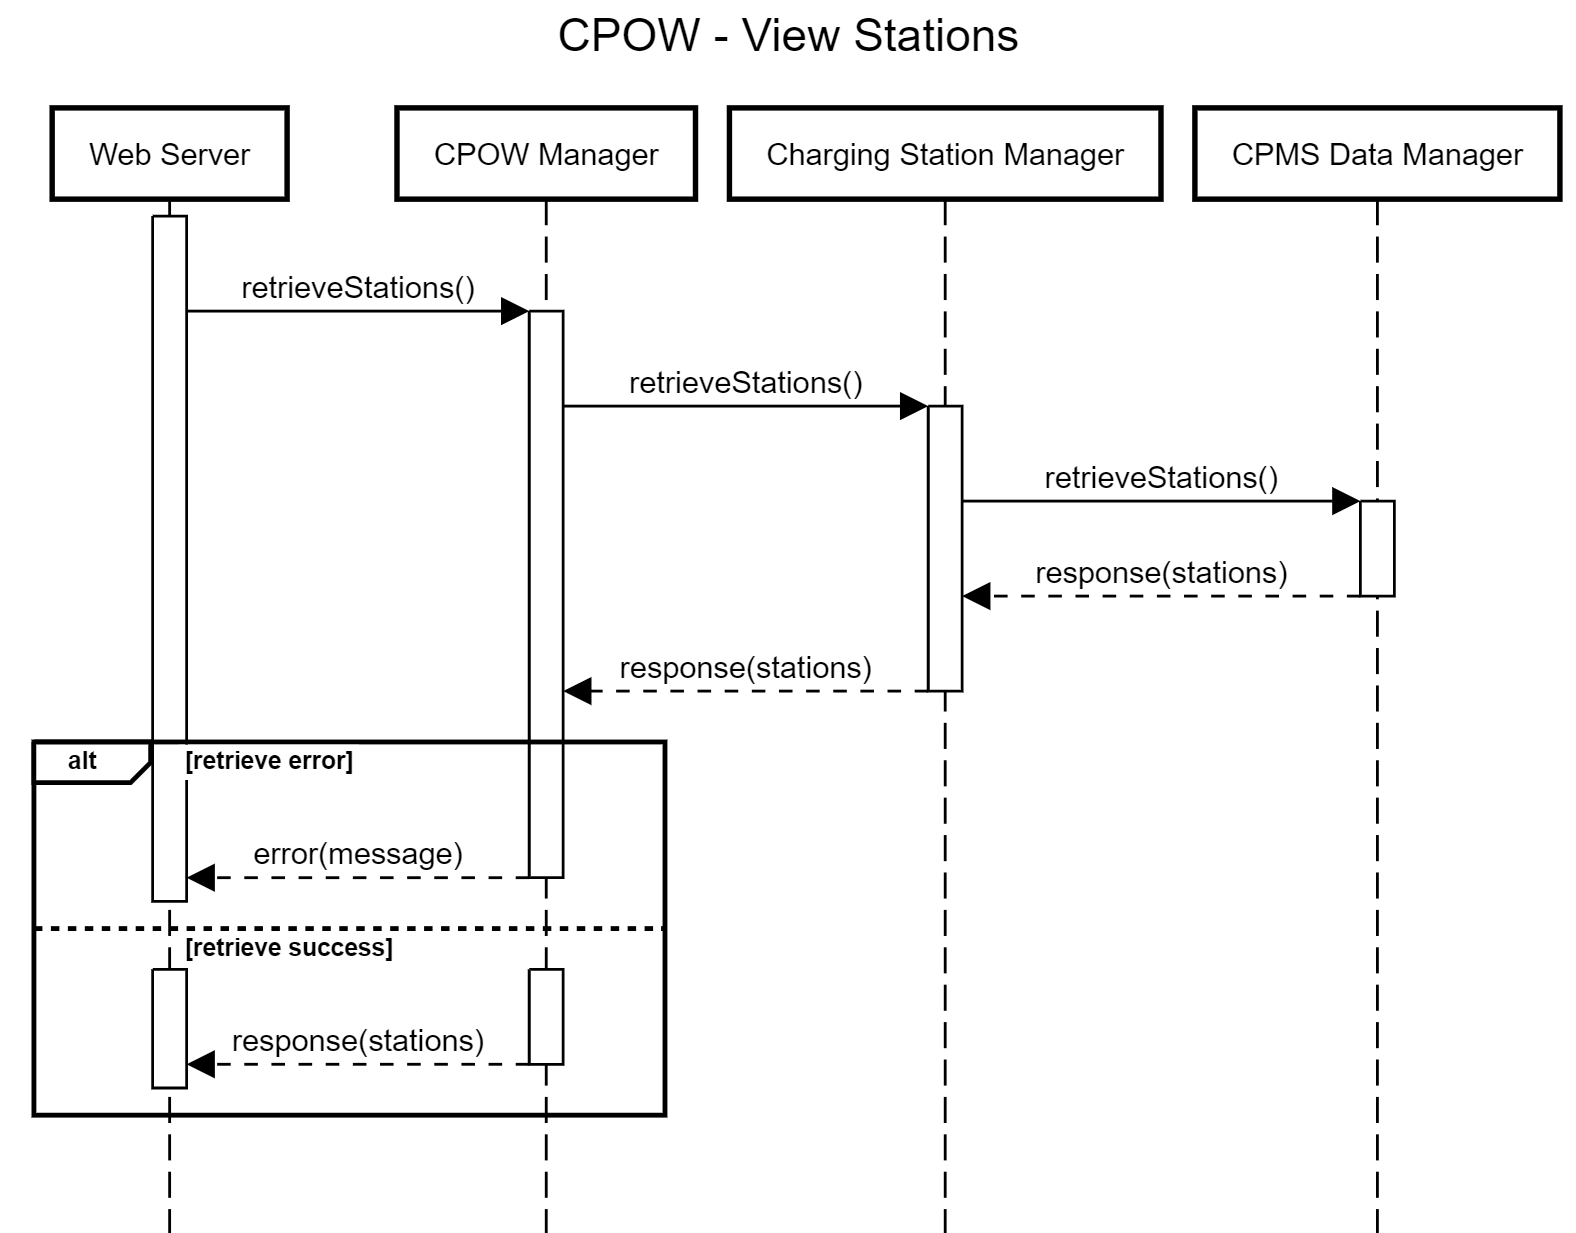
\includegraphics[scale=0.25, center]{assets/sequenceDiagrams/CPOW view stations.png}
        \caption{CPOW - View charging stations}
        \label{CPOW - View charging stations}
    \end{figure}
\end{center}
This diagram describes the data fetching interaction between the Web Server and the Applicantion Server in order to retrieve the list of charging stations that are connected to the CPMS.
The list will contain all the stations details, such as the ID, the location, the energy provider, the status and the socket details and a button to change the energy provider.
\newpage

\textbf{Change energy provider}
\begin{center}
    \begin{figure}[H]
        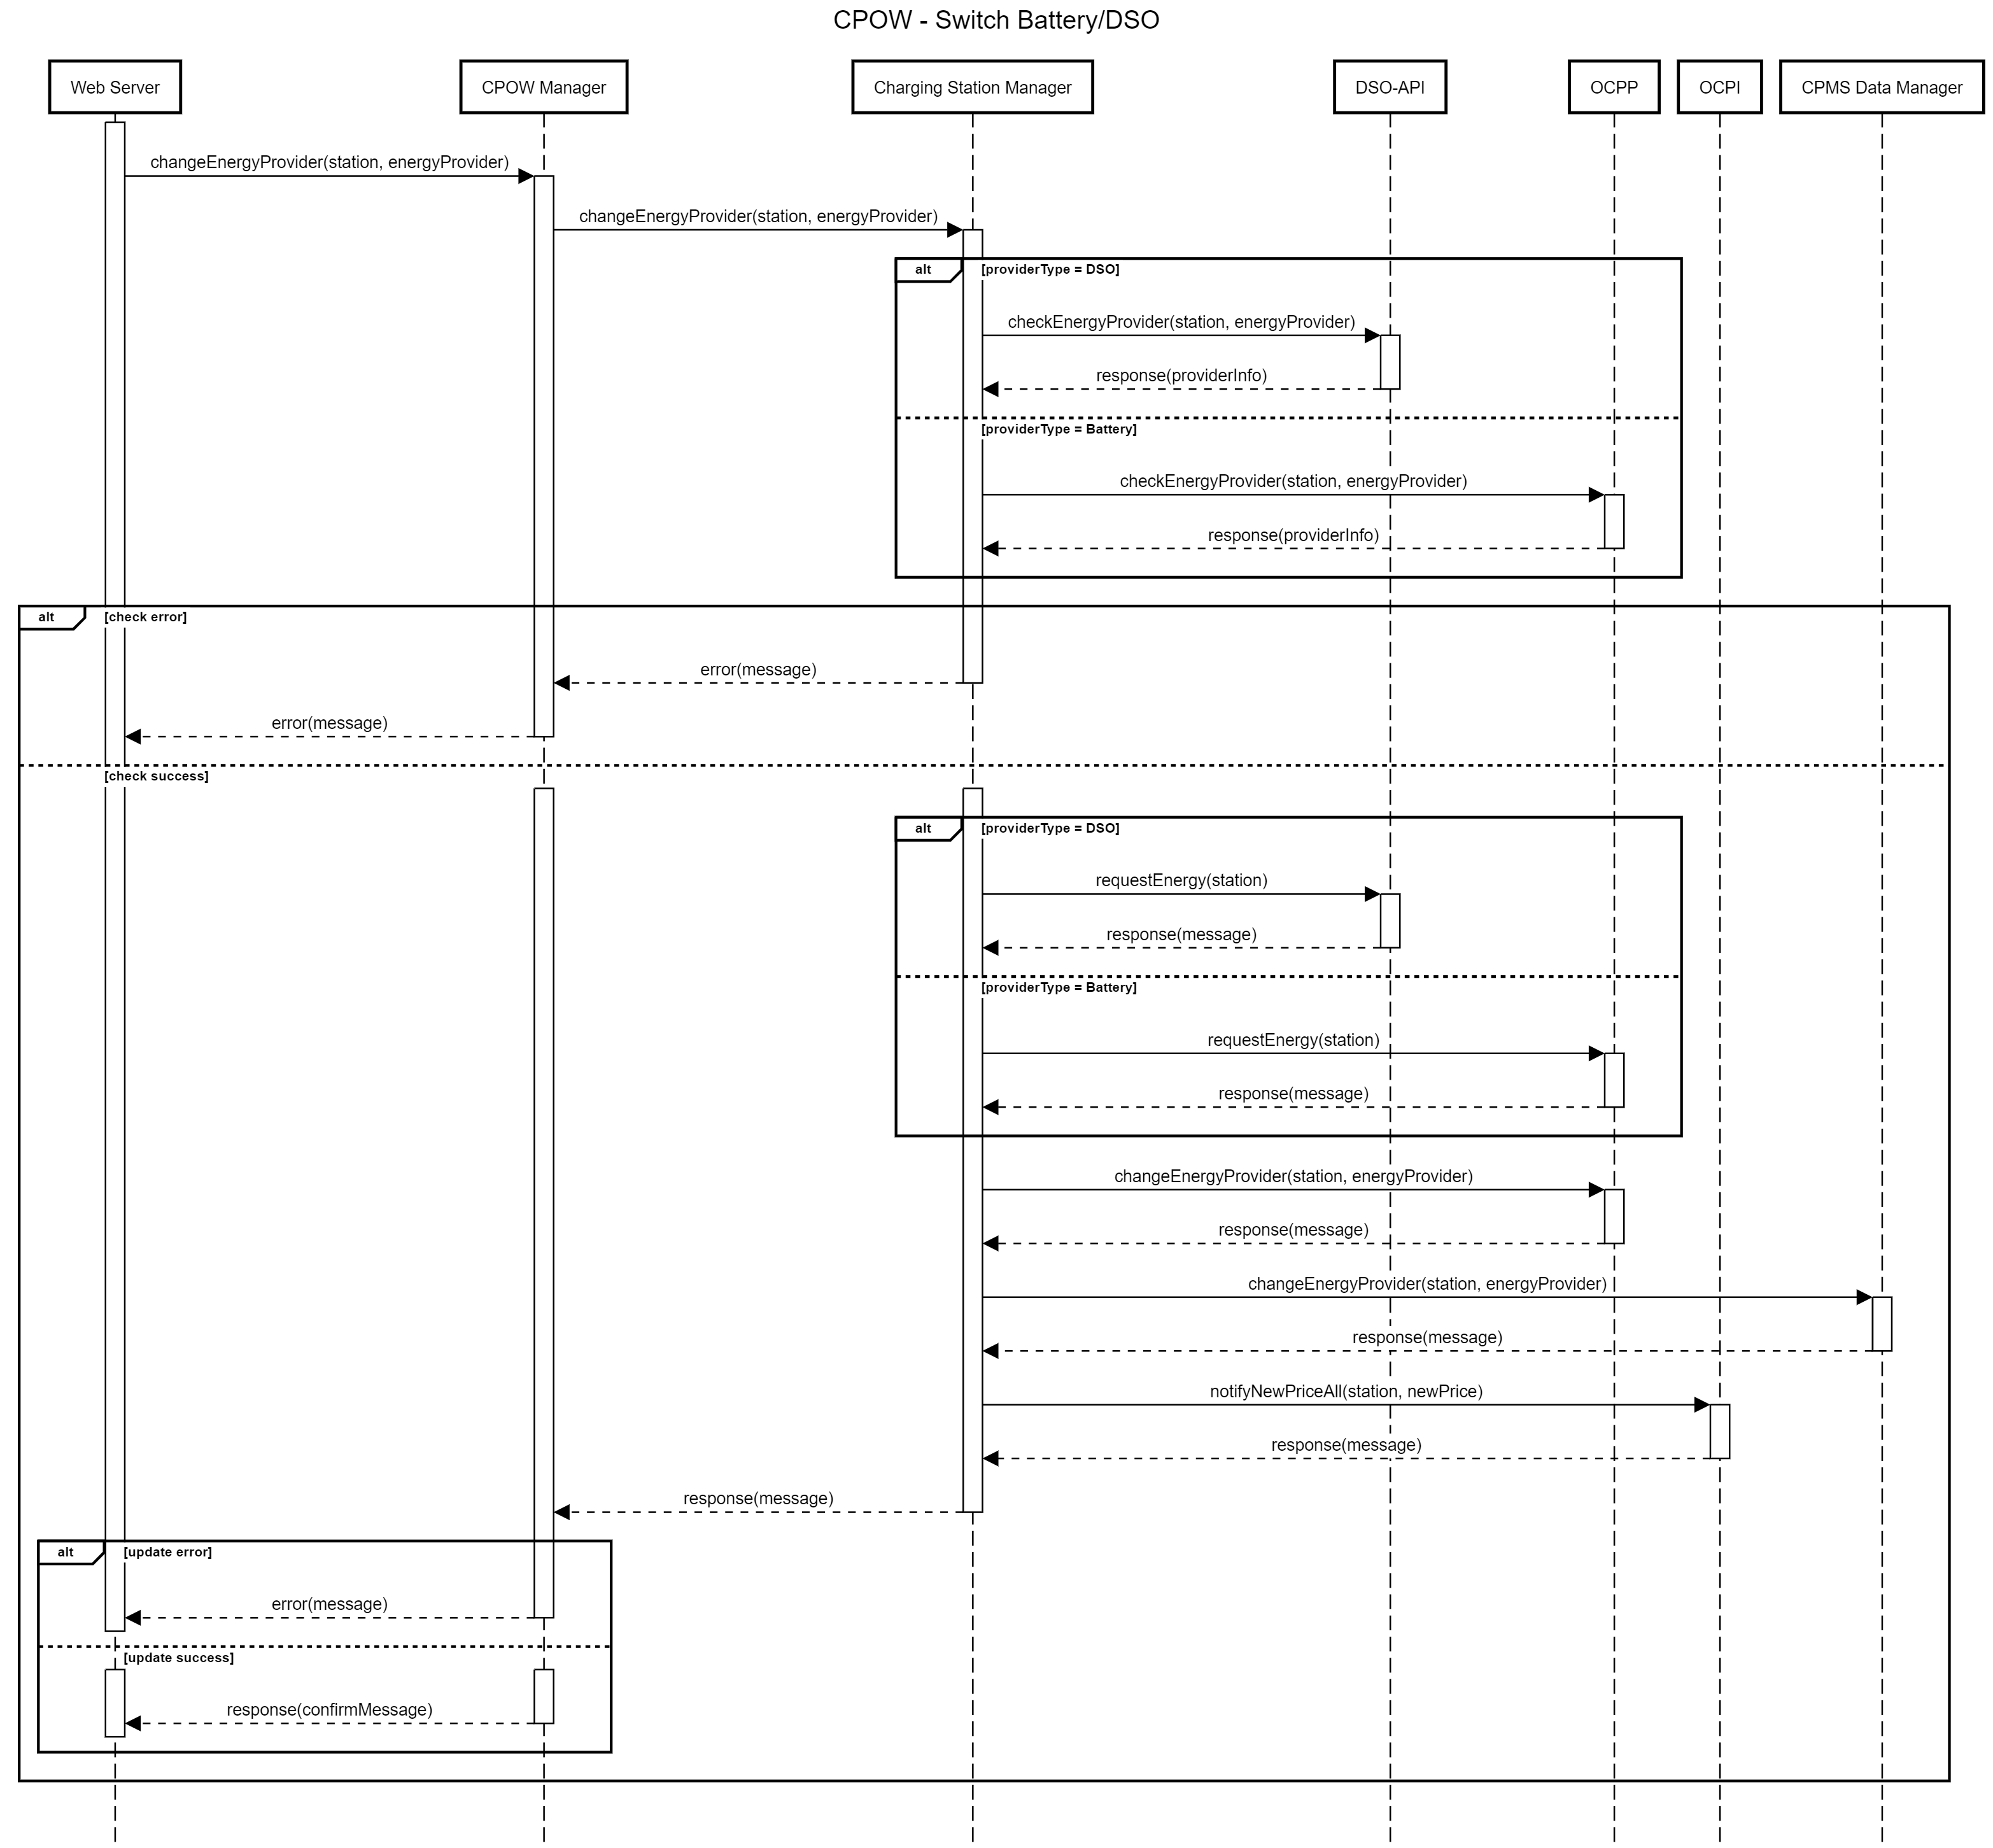
\includegraphics[scale=0.15, center]{assets/sequenceDiagrams/CPOW change energy.png}
        \caption{CPOW - Change energy provider}
        \label{CPOW - Change energy provider}
    \end{figure}
\end{center}
\newpage
This diagram describes the interaction between the CPOW and the Applicantion Server in order to change the energy provider of a charging station.\\
It starts by the CPOW sending a request with the charging station ID and the new energy provider (after retrieving a list with all the stations details, described in Figure \ref*{CPOW - View charging stations}).
Then, the Charging Station Manager will check if the station exists and if the energy provider is valid by communicating with the OCPP or the DSP-API component, depending if the selected provider is a DSO or an internal battery.
If the selected provider is available, the Charging Station Manager will ask the Provider to start supplying the energy, notify the station through OCPP, notify the connected eMSPs through OCPI, and update the station's current energy provider in the database.
\newpage


\subsection{Component interfaces}

\begin{center}
    \begin{figure}[H]
        
\includegraphics[scale=0.60, center]{assets/placeholder.png}
        \caption{Component Interfaces Diagram}
        \label{fig: component_interfaces}
    \end{figure}
\end{center}

This diagram above describes in detail the interfaces and the corresponding methods offered by each component, it also shows the interaction between them.
*other text*

\subsection{Selected architectural styles and patterns}

    \begin{itemize}
        \item \textbf{type of architecture} \newline
             description and reasoning
        \item \textbf{Type of client} \newline
              description and reasoning
        \item \textbf{Scalability} \newline
              how can the architecture manage help scalability
        \item \textbf{MVC?} \newline
              general description
              \begin{itemize}
                  \item Model: the central component of the pattern. It is the application's dynamic data structure, independent of the user interface. It directly manages the data, logic and rules of the application.
                  \item View: The view defines how the app's data should be displayed.
                  \item Controller: it contains logic that updates the model and/or view in response to input from the users of the app. 
              \end{itemize}
    \end{itemize}

\newpage


\subsection{Other design decisions}
\label{other_design_decisions}
\subsubsection{Servers availability and response time} 
\label{server_availability}
text
\subsubsection{exaple of design decision} 
description of example

\begin{equation}
    possible\  equation \ to \ be \  included 
\end{equation}

development of said equation 

\begin{align}  
    description\ of\ development\ pt1\
    description\ of\ development\ pt2
\end{align}

other development and various considerations

%\begin{testexample}
%example of an application of our design decision (with data)
%\end{testexample}

 conclusion of design decision

 \subsubsection{design decision 2} 
    \begin{itemize}
        \item text
    \end{itemize}

\subsubsection{design decision 3} text

\newpage

\section{User Interface Design}
\begin{center}
    \begin{figure}[H]
        
\includegraphics[scale=0.74, center]{assets/placeholder.png}
        \caption{Sign Up and Log In}
        \label{fig: signMockup}
    \end{figure}
\end{center}

\begin{center}
    \begin{figure}[H]
        \vspace{-50px}
        
\includegraphics[scale=0.6, center]{assets/placeholder.png}
        \caption{carOwner interactions}
        \label{fig: agroMockup}
    \end{figure}
\end{center}

\begin{center}
    \begin{figure}[H]
        
\includegraphics[scale=0.6, center]{assets/placeholder.png}
        \caption{CPOW interactions}
        \label{fig: farmerInter}
    \end{figure}
\end{center}

\newpage

\section{Requirements Traceability}

\begin{longtable}{|p{0.47\textwidth}|p{0.45\textwidth}|}
    \hline
    \textbf{Requirements} & \textbf{Components} \\\hline\hline
    \begin{itemize}
        \item[R1)] text.
        \item[R2)] text.
        \item[R3)] text.
    \end{itemize}
    & 
    \begin{itemize}
        \item text.
        \item text.
        \item text.
    \end{itemize}
    \\\hline

    \begin{itemize}
        \item[R4)] text.
    \end{itemize}
    & 
    \begin{itemize}
        \item text.
    \end{itemize}
    \\\hline

    \begin{itemize}
        \item[R5)] text.
        \item[R6)] text.
        \item[R7)] text.
    \end{itemize}
    & 
    \begin{itemize}
        \item text.
        \begin{itemize}
            \setlength{\itemindent}{-5px}
            \item text.
            \item text.
            \item text.
        \end{itemize}
        \item text.
        \item text.
        \item text.
        \item text.
    \end{itemize}
    \\\hline

    \begin{itemize}
        \item[R8)] text.
    \end{itemize}
    & 
    \begin{itemize}
        \item text.
    \end{itemize}
    \\\hline

    \begin{itemize}
        \item[R9)] text.
    \end{itemize}
    &
    \begin{itemize}
        \item text.
        \begin{itemize}
            \item text.
        \end{itemize}
        \item text.
    \end{itemize}
    \\\hline

    \begin{itemize}
        \item[R10)] text.
    \end{itemize}
    &
    \begin{itemize}
        \item text.
        \begin{itemize}
            \item text.
        \end{itemize}
        \item text.
        \item text.
        \item text.
    \end{itemize}
    \\\hline

    \begin{itemize}
        \item[R11)] text.
    \end{itemize}
    &
    \begin{itemize}
        \item text.
        \begin{itemize}
            \item text.
        \end{itemize}
        \item text.
        \item text.
    \end{itemize}
    \\\hline

    \begin{itemize}
        \item[R12)] text.
    \end{itemize}
    &
    \begin{itemize}
        \item text.
        \begin{itemize}
            \item text.
        \end{itemize}
        \item text.
    \end{itemize}
    \\\hline

    \begin{itemize}
        \item[R13)] text.
        \item[R14)] text.
        \item[R15)] text. 
        \item[R16)] text.
        \item[R17)] text. 
    \end{itemize}

    &
    \begin{itemize}
        \item text. \begin{itemize}
            \item text.
        \end{itemize}
    \end{itemize}
    \\\hline

    \begin{itemize}
        \item[R18)] text.
    \end{itemize}
    &
    \begin{itemize}
        \item text. 
        \item text.
        \begin{itemize}
            \item text.
        \end{itemize}
    \end{itemize}
    \\\hline

    \begin{itemize}
        \item[R19)] text.
    \end{itemize}
    &
    \begin{itemize}
        \item text.
        \item text.
        \item text.
    \end{itemize}
    \\\hline

    \begin{itemize}
        \item[R20)] text. 
    \end{itemize}
    &
    \begin{itemize}
        \item text.
        \item text.
    \end{itemize}
    \\\hline
    \begin{itemize}
        \item[R21)] text.
    \end{itemize}
    &
    \begin{itemize}
        \item text.
    \end{itemize}\\\hline
\end{longtable}

Here, we present a summary of the table above for a more immediate visualization.
*component: name associated in the next table*
\begin{table}[H]
    \centering
    \begin{tabular}{|l l|}
        \hline
        component 1:& c1\\
        component 2:& c2\\\hline
        
    \end{tabular}
    \caption{Components' legend}
\end{table}
\newpage
\setlength\LTleft{-2.5cm}
\begin{longtable}{|c|c|c|}

    \hline
    & \cellcolor{blue!30}c1 & \cellcolor{blue!30}c2 \\\hline
    \cellcolor{SpringGreen!50}R1 & x & x \\\hline
    \cellcolor{SpringGreen!50}R2 & x & x \\\hline
    \cellcolor{SpringGreen!50}R3 & x & x \\\hline
    \cellcolor{SpringGreen!50}R4 & x &  \\\hline
    \cellcolor{SpringGreen!50}R5 &    & \\\hline
    \cellcolor{SpringGreen!50}R6 &    & \\\hline
    \cellcolor{SpringGreen!50}R7 &    & \\\hline
    \cellcolor{SpringGreen!50}R8 &    & \\\hline
    \cellcolor{SpringGreen!50}R9 &    & \\\hline
    \cellcolor{SpringGreen!50}R10 &    & \\\hline
    \cellcolor{SpringGreen!50}R11 &    & \\\hline
    \cellcolor{SpringGreen!50}R12 &    & \\\hline
    \cellcolor{SpringGreen!50}R13 &    & \\\hline
    \cellcolor{SpringGreen!50}R14 &    & \\\hline
    \cellcolor{SpringGreen!50}R15 &    & \\\hline
    \cellcolor{SpringGreen!50}R16 &    & \\\hline
    \cellcolor{SpringGreen!50}R17 &    & \\\hline
    \cellcolor{SpringGreen!50}R18 &    & \\\hline
    \cellcolor{SpringGreen!50}R19 &    & \\\hline
    \cellcolor{SpringGreen!50}R20 &    & \\\hline
    \cellcolor{SpringGreen!50}R21 & &\\\hline
    \caption{Component and requirement mapping}\\
\end{longtable}

\section{Implementation, Integration and Test Plan}
\subsection{Implementation Plan}
Multiple components will be implemented at the same time, in order to parallelize the development when possible. The general plan is to follow a bottom-up approach, so that core and basic functionalities with very few dependencies can be tested as soon as their incapsulating component is done. By doing so, the application will be built up with solid and tested foundations that will ease the further testing of bigger and complex components. In any case, unit testing will be performed on each component on the go, in order to find flaws out in advance. This will positevely impact the necessary actions to fix the faults since they will be done in an earlier stage.

The implementation's order of the component will be as follow:
\begin{enumerate}
    \item list, of, components
    \item list, of, components, 2
    \item list, of, components, 3
\end{enumerate}
Each group is composed by independent modules so they can be easily developed in parallel.
Furthermore, it is expected that external services (e.g. GoogleMapsAPI, *others* and DBMS Service) work properly since they're not a responsibility of the *name* app.

*explanation of the implementation plan component order*
\subsection{Integration Strategy}
Considering both the overall system's architecture and the implementation
plan, the chosen integration strategy is the bottom-up approach. System
integration begins with the integration of the lowest level modules and uses
test drivers to drive and pass appropriate data to the lower-level modules. As
and when the code for the other module gets ready, these drivers are replaced
with the actual module.

This approach allows to start the integration and testing without necessarily
waiting for the completion of the development and the unit testing of each
system's component. Being the low-level modules and their combined functions
often invoked by other modules, it is more useful to test them first so that
meaningful effective integration of other modules can be done. Moreover,
starting at the bottom of the hierarchy means that the critical modules are built
and tested first and therefore any errors in these modules are identified early in
the process.

Each integration in the same level (defined by the groups of the previous
section) is independent and there is no specific order in which to complete them.
In this way, the integration process and its testing are more flexible.

\subsubsection{Integration and Testing}
In this section it is defined the order of the integration between components. Test drivers will be used to simulate higher components not yet implemented.
*order of the components shown in the next figures, with references*

\begin{figure}[H]
    
\includegraphics[scale=0.6, center]{assets/placeholder.png}
    \caption{Integration of first component}
    \label{fig: integration_DataManager}
\end{figure}

\begin{figure}[H]
    \centering
    
\includegraphics[scale=0.6]{assets/placeholder.png} 
    \caption{Integration of second component}%
    \label{fig: integration_MapServiceManager_WeatherManager}%
\end{figure}

\begin{figure}[H]
    \centering
    \subfloat[\centering component 3a]{{
\includegraphics[scale=0.5]{assets/placeholder.png}}}%
    \qquad\qquad
    \subfloat[\centering component 3b]{{
\includegraphics[scale=0.5]{assets/placeholder.png}}}%
    \caption{Integration of 3a and 3b components}%
    \label{fig: integration_SensorDataManager_NewsManager}%
\end{figure}

*order of components for the middle tier, with references*
\begin{figure}[H]
    \centering
    \subfloat[\centering component middle1-a]{{
\includegraphics[scale=0.5]{assets/placeholder.png}}}%
    \qquad\qquad
    \subfloat[\centering component middle1-b]{{
\includegraphics[scale=0.5]{assets/placeholder.png}}}%
    \qquad\qquad
    \subfloat[\centering component middle1-c]{{
\includegraphics[scale=0.7]{assets/placeholder.png}}}%
    \caption{Integration of middle1-a,b,c components}%
    \label{fig: integration_RankingManager_HelpRequestManager}%
\end{figure}
\begin{figure}[H]
    \centering
    
\includegraphics[scale=0.55]{assets/placeholder.png}%
    \caption{Integration of middle2 component}%
    \label{fig: integration_ForumManager_LocationModule}%
\end{figure}

*order of last group components, with references to the images*

\begin{figure}[H]
    \centering
    
\includegraphics[scale=0.6, center]{assets/placeholder.png}
    \caption{Integration of carOwnerManager components}
    \label{fig: integration_PolicyMakerManager}
\end{figure}
\begin{figure}[H]
    \centering
    
\includegraphics[scale=0.6, center]{assets/placeholder.png}
    \caption{Integration CPOWmanager components}
    \label{fig: integration_AgronomistManager}
\end{figure}
\begin{figure}[H]
    \centering
    
\includegraphics[scale=0.6, center]{assets/placeholder.png}
    \caption{Integration of otherManager components}
    \label{fig: integration_FarmerManager}
\end{figure}
\begin{figure}[H]
    \centering
    
\includegraphics[scale=0.7, center]{assets/placeholder.png}
    \caption{Integration of AccountManager components}
    \label{fig: integration_AccountManager}
\end{figure}

\subsection{System testing}
*text for sys testing*
\newpage
\section{Effort Spent}
    \begin{tabular}{|c||c|c|c|c|c|}
        \hline
        Student & Time for S.1 & S.2 & S.3 & S.4 & S.5\\ \hline
        stud1 & 0h & 0h & 0h & 0h & 0h \\
        stud2 & 0h & 0h & 0h & 0h & 0h \\
        stud3 & 0h & 0h & 0h & 0h & 0h \\
        \hline
    \end{tabular}


\section{References}


\begin{thebibliography}{9}
    \bibitem{reference1}
    MDN Web Docs Glossary: Definitions of Web-related terms -> MVC
    \url{https://developer.mozilla.org/en-US/docs/Glossary/MVC}

    \bibitem{reference2}
    description: \url{url here}
    
\end{thebibliography}

\end{document}